% Template for PLoS
% Version 3.4 January 2017
%
% % % % % % % % % % % % % % % % % % % % % %
%
% -- IMPORTANT NOTE
%
% This template contains comments intended
% to minimize problems and delays during our production
% process. Please follow the template instructions
% whenever possible.
%
% % % % % % % % % % % % % % % % % % % % % % %
%
% Once your paper is accepted for publication,
% PLEASE REMOVE ALL TRACKED CHANGES in this file
% and leave only the final text of your manuscript.
% PLOS recommends the use of latexdiff to track changes during review, as this will help to maintain a clean tex file.
% Visit https://www.ctan.org/pkg/latexdiff?lang=en for info or contact us at latex@plos.org.
%
%
% There are no restrictions on package use within the LaTeX files except that
% no packages listed in the template may be deleted.
%
% Please do not include colors or graphics in the text.
%
% The manuscript LaTeX source should be contained within a single file (do not use \input, \externaldocument, or similar commands).
%
% % % % % % % % % % % % % % % % % % % % % % %
%
% -- FIGURES AND TABLES
%
% Please include tables/figure captions directly after the paragraph where they are first cited in the text.
%
% DO NOT INCLUDE GRAPHICS IN YOUR MANUSCRIPT
% - Figures should be uploaded separately from your manuscript file.
% - Figures generated using LaTeX should be extracted and removed from the PDF before submission.
% - Figures containing multiple panels/subfigures must be combined into one image file before submission.
% For figure citations, please use "Fig" instead of "Figure".
% See http://journals.plos.org/plosone/s/figures for PLOS figure guidelines.
%
% Tables should be cell-based and may not contain:
% - spacing/line breaks within cells to alter layout or alignment
% - do not nest tabular environments (no tabular environments within tabular environments)
% - no graphics or colored text (cell background color/shading OK)
% See http://journals.plos.org/plosone/s/tables for table guidelines.
%
% For tables that exceed the width of the text column, use the adjustwidth environment as illustrated in the example table in text below.
%
% % % % % % % % % % % % % % % % % % % % % % % %
%
% -- EQUATIONS, MATH SYMBOLS, SUBSCRIPTS, AND SUPERSCRIPTS
%
% IMPORTANT
% Below are a few tips to help format your equations and other special characters according to our specifications. For more tips to help reduce the possibility of formatting errors during conversion, please see our LaTeX guidelines at http://journals.plos.org/plosone/s/latex
%
% For inline equations, please be sure to include all portions of an equation in the math environment.  For example, x$^2$ is incorrect; this should be formatted as $x^2$ (or $\mathrm{x}^2$ if the romanized font is desired).
%
% Do not include text that is not math in the math environment. For example, CO2 should be written as CO\textsubscript{2} instead of CO$_2$.
%
% Please add line breaks to long display equations when possible in order to fit size of the column.
%
% For inline equations, please do not include punctuation (commas, etc) within the math environment unless this is part of the equation.
%
% When adding superscript or subscripts outside of brackets/braces, please group using {}.  For example, change "[U(D,E,\gamma)]^2" to "{[U(D,E,\gamma)]}^2".
%
% Do not use \cal for caligraphic font.  Instead, use \mathcal{}
%
% % % % % % % % % % % % % % % % % % % % % % % %
%
% Please contact latex@plos.org with any questions.
%
% % % % % % % % % % % % % % % % % % % % % % % %

\documentclass[10pt,letterpaper]{article}
\usepackage[top=0.85in,left=2.75in,footskip=0.75in]{geometry}

% amsmath and amssymb packages, useful for mathematical formulas and symbols
\usepackage{amsmath,amssymb}

% Use adjustwidth environment to exceed column width (see example table in text)
\usepackage{changepage}

% Use Unicode characters when possible
\usepackage[utf8x]{inputenc}

% textcomp package and marvosym package for additional characters
\usepackage{textcomp,marvosym}

% cite package, to clean up citations in the main text. Do not remove.
\usepackage{cite}

% Use nameref to cite supporting information files (see Supporting Information section for more info)
\usepackage{nameref,hyperref}

% line numbers
\usepackage[right]{lineno}

% ligatures disabled
\usepackage{microtype}
\DisableLigatures[f]{encoding = *, family = * }

% color can be used to apply background shading to table cells only
\usepackage[table]{xcolor}

% array package and thick rules for tables
\usepackage{array}

% create "+" rule type for thick vertical lines
\newcolumntype{+}{!{\vrule width 2pt}}

% create \thickcline for thick horizontal lines of variable length
\newlength\savedwidth
\newcommand\thickcline[1]{%
  \noalign{\global\savedwidth\arrayrulewidth\global\arrayrulewidth 2pt}%
  \cline{#1}%
  \noalign{\vskip\arrayrulewidth}%
  \noalign{\global\arrayrulewidth\savedwidth}%
}

% \thickhline command for thick horizontal lines that span the table
\newcommand\thickhline{\noalign{\global\savedwidth\arrayrulewidth\global\arrayrulewidth 2pt}%
\hline
\noalign{\global\arrayrulewidth\savedwidth}}


% Remove comment for double spacing
%\usepackage{setspace}
%\doublespacing

% Text layout
\raggedright
\setlength{\parindent}{0.5cm}
\textwidth 5.25in
\textheight 8.75in

% Bold the 'Figure #' in the caption and separate it from the title/caption with a period
% Captions will be left justified
\usepackage[aboveskip=1pt,labelfont=bf,labelsep=period,justification=raggedright,singlelinecheck=off]{caption}
\renewcommand{\figurename}{Fig}

% Use the PLoS provided BiBTeX style
\bibliographystyle{plos2015}

% Remove brackets from numbering in List of References
\makeatletter
\renewcommand{\@biblabel}[1]{\quad#1.}
\makeatother

% Leave date blank
\date{}

% Header and Footer with logo
\usepackage{lastpage,fancyhdr,graphicx}
\usepackage{epstopdf}
\pagestyle{myheadings}
\pagestyle{fancy}
\fancyhf{}
\setlength{\headheight}{27.023pt}
% \lhead{
\includegraphics[width=2.0in]{PLOS-submission.eps}}
\rfoot{\thepage/\pageref{LastPage}}
\renewcommand{\footrule}{\hrule height 2pt \vspace{2mm}}
\fancyheadoffset[L]{2.25in}
\fancyfootoffset[L]{2.25in}
% \lfoot{\sf PLOS}

%% Include all macros below

%\newcommand{\lorem}{{\bf LOREM}}
%\newcommand{\ipsum}{{\bf IPSUM}}

%% END MACROS SECTION


\begin{document}
\vspace*{0.2in}

% Title must be 250 characters or less.
\begin{flushleft}
{\Large
\textbf\newline{Elucidating multi-input processing 3-node gene regulatory
network topologies capable of generating striped gene expression patterns}
% Please use "sentence case" for title and headings (capitalize only the first word in a title (or heading), the first word in a subtitle (or subheading), and any proper nouns).
}
\newline
% Insert author names, affiliations and corresponding author email (do not include titles, positions, or degrees).
\\
Juan Camilo Arboleda-Rivera\textsuperscript{1*},
Gloria Machado-Rodríguez\textsuperscript{1},
Boris A. Rodríguez\textsuperscript{2},
Jayson Gutiérrez\textsuperscript{3},
% Name5 Surname\textsuperscript{2\ddag},
% Name6 Surname\textsuperscript{2\ddag},
% Name7 Surname\textsuperscript{1,2,3*},
% with the Lorem Ipsum Consortium\textsuperscript{\textpilcrow}
\\
\bigskip
\textbf{1} Grupo de Fundamentos y Enseñanza de la Física y los Sistemas Dinámicos,
Instituto de Biología, Facultad de Ciencias Exactas y Naturales, Universidad de Antioquia
UdeA, Calle 70 No. 52-21, Medellín, Colombia.
\\
\textbf{2} Grupo de Fundamentos y Enseñanza de la Física y los Sistemas Dinámicos,
Instituto de Física, Facultad de Ciencias Exactas y Naturales, Universidad de Antioquia
UdeA, Calle 70 No. 52-21, Medellín, Colombia.
\\
\textbf{3} Flanders Marine Institute (VLIZ), Wandelaarkaai 7, 8400 Oostende,
Belgium
% \textbf{3} Affiliation Dept/Program/Center, Institution Name, City, State, Country
\\
\bigskip

% Insert additional author notes using the symbols described below. Insert symbol callouts after author names as necessary.
%
% Remove or comment out the author notes below if they aren't used.
%
% Primary Equal Contribution Note
% \Yinyang These authors contributed equally to this work.

% Additional Equal Contribution Note
% Also use this double-dagger symbol for special authorship notes, such as senior authorship.
% \ddag These authors also contributed equally to this work.

% Current address notes
% \textcurrency Current Address: Dept/Program/Center, Universidad de Antioquia,
% Medellín, Antioquia, Colombia % change symbol to "\textcurrency a" if more than one current address note
% \textcurrency b Insert second current address
% \textcurrency c Insert third current address

% Deceased author note
% \dag Deceased

% Group/Consortium Author Note
% \textpilcrow Membership list can be found in the Acknowledgments section.

% Use the asterisk to denote corresponding authorship and provide email address in note below.
* juan.arboleda2@udea.edu.co

\end{flushleft}
% Please keep the abstract below 300 words
\section*{Abstract}

\subsection*{Background}
A central problem in developmental and synthetic biology is understanding the
mechanisms by which cells in a tissue or a Petri dish process external cues
and transform such information into a coherent response, e.g., a terminal
differentiation state. It was long believed that this type of positional
information could be entirely attributed to a gradient of concentration of a
specific signaling molecule (i.e., a morphogen). However, advances in experimental
methodologies and computer modeling have demonstrated the crucial role of the
dynamics of a cell's gene regulatory network (GRN) in decoding the information
carried by the morphogen, which is eventually translated into a spatial
pattern. This morphogen interpretation mechanism has gained much attention
in systems biology as a tractable system to investigate the emergent properties
of complex genotype-phenotype maps.

\subsection*{Methods}
In this study, we apply a Markov chain Monte Carlo (MCMC)-like algorithm to probe
the design space of three-node GRNs with the ability to generate a band-like
expression pattern (target phenotype) in the middle of an arrangement of 30
cells, which resemble a simple (1-D) morphogenetic field in a developing embryo.
Unlike most modeling studies published so far, here we explore the
space of GRN topologies with nodes having the potential to perceive
the same input signal differently. This allows for a lot more flexibility during the search
space process, and thus enables us to identify a larger set of potentially
interesting and realizable morphogen interpretation mechanisms.

\subsection*{Results}
Out of 2061 GRNs selected using the search space algorithm, we found 714 classes of
network topologies that could correctly interpret the morphogen.
Notably, the main network motif that generated the target phenotype in
response to the input signal was the type 3 Incoherent Feed-Forward Loop (I3-FFL),
which agrees with previous theoretical expectations and experimental
observations. Particularly, compared to a previously reported pattern forming GRN
topologies, we have uncovered a great variety of novel network designs, some of
which might be worth inquiring through synthetic biology methodologies to test
for the ability of network design with minimal regulatory complexity to
interpret a developmental cue robustly.


% \subsection*{Conclusions}

% Please keep the Author Summary between 150 and 200 words
% Use first person. PLOS ONE authors please skip this step.
% Author Summary not valid for PLOS ONE submissions.
\section*{Author summary}
Systems biology is a fast growing field largely powered by advances in
high-performance computing and sophisticated mathematical modeling of
biological systems. Based on these advances, we are now in a position to
mechanistically understand and accurately predict the behavior of
complex biological processes, including cell differentiation and spatial pattern
formation during embryogenesis. In this article, we use an \textit{in silico}
approach to probe the design space of multi-input, three-node Gene Regulatory
Networks (GRNs) capable of generating a striped gene expression pattern in
the context of a simplified 1-D morphogenetic field.

\linenumbers

% Use "Eq" instead of "Equation" for equation citations.
\section*{Introduction}

Cells interact continuously with their environment, which requires precise
regulatory strategies to avoid potential detrimental responses. Arguably, most
cellular functions arise from the dynamic activity of Gene Regulatory Networks
(GRNs), which play a central role in interpreting external and internal
signals. This information processing function is critical in
developmental processes such as those in which a group of cells differentiates in
response to a signaling molecule. Such molecules were referred to as morphogens by Turing in
1952~\cite{Turing1952}, and posterior theoretical studies on patterning led to the
conceptualization of the French Flag Problem by Wolpert, who also stated
in this respect that a gradient of concentration of a morphogen could
trigger cell differentiation in a one-dimensional field of cells~\cite{Wolpert1969,
sharpe_2019}.
Although the Bicoid protein (bcd), the first example of a molecule that acted
as a morphogen, was only found in the 80s in the developing embryos of
\textit{Drosophila melanogaster}~\cite{driever_gradient_1988,
driever_bicoid_1988}, now it is known that there
are many other examples such as the Decapentaplegic (Dpp) protein in
\textit{Drosophila} wing imaginal discs~\cite{affolter_decapentaplegic_2007},
as well as Sonic Hedgehog~\cite{dessaud_dynamic_2010,cohen_theoretical_2014}
and Wnt~\cite{raspopovic_digit_2014}. However, information processing by GRNs
has proven to be a complex process, and a major goal of developmental biology
is to understand mechanistically how positional information conveyed by morphogens
is translated into spatial differentiation.\\

Our understanding of how GRNs process information has increased thanks to the
concept and theory of network motifs, defined as patterns of
interconnections occurring in networks at numbers significantly higher
than those in randomized networks~\cite{Milo2002}. This novel approach, along
with mathematical modeling and computational systems biology methods, is a
powerful tool to study GRNs~\cite{kitano_computational_2002}, and
experimental studies have validated the predictions of studies using these
methods~\cite{Kalir2005,Kalir2004,Mangan2003a,ODonnell2005}.
Some have even used synthetic GRNs to produce artificial cell
differentiation~\cite{Basu2005}, circadian gene
expression~\cite{atkinson_development_2003}, counting
devices~\cite{friedland_synthetic_2009} and systems that respond to
light~\cite{gardner2012,levskaya2005}.
Moreover, the design and implementation of GRNs through synthetic biology is
emerging as a promising tool to study biological phenomena as pattern
formation~\cite{santos-moreno_using_2019} and as a novel therapeutic tool with
interesting biomedical applications~\cite{karlsson_therapeutic_2012,
higashikuni_advancing_2017,abil_synthetic_2015,healy_genetic_2019,
kitada_programming_2018}.

In a tissue context, the generation of a stripe of gene expression is a fundamental
patterning function in development, and it has been shown that simple feed-forward
motifs can robustly achieve such a patterning task~\cite{munteanu_2014}. For
example, Cotterell and Sharpe studied what kind of 3-node network topologies
could effectively translate a morphogen gradient into a striped gene expression
pattern in a one-dimensional field of cells. They found a variety of networks that
implemented at least 7 different mechanisms with varying complexity levels,
most of them variations of feed-forward motifs~\cite{Cotterell2010}.

Although GRNs with positional information processing capacities have been
extensively analyzed, most studies have so far emphasized particular
regulatory systems that respond to a single input only. These studies have
typically focused on either regulatory systems observed in
nature~\cite{vonDassow2000,Reinitz1995,Jaeger2004}, synthetic
implementations with predefined topologies~\cite{Basu2005, Schaerli2018,
Elowitz2000, barbier2020}, or have deliberately constrained the study of GRNs to just
a handful of alternative designs~\cite{munteanu_2014,Schaerli2014}. However,
previous work has demonstrated the necessity to expand computational analysis
of pattern forming GRNs to multi-input settings. For instance, it has been shown
that the neural subtypes specification system in the vertebrate neural tube involves
a  two-input network in which Sonic Hedgehog acts as a morphogen and the Olig2
and Nkx2.2 genes can act as the receiver nodes~\cite{dessaud_dynamic_2010,
balaskas2012, exelby_2021}.

In this study, we apply a Markov chain Monte Carlo (MCMC)-like algorithm to
probe the design space of three-node GRNs looking for topologies capable of
translating a morphogen gradient  (input signal) into a striped pattern of gene
expression (phenotype). Importantly, unlike most previous computational
studies, here we allowed any node (e.g., gene) in a GRN to perceive the input
signal in varying ways and selected the best-performing GRNs based on a
fitness criterion used to assess the quality of the phenotype with respect to
a prescribed optimal pattern. Based on this computational strategy, we uncovered
a great variety of distinct classes of network topologies that
tend to form a complex interconnected meta-graph that could be easily
traversed throughout evolution via single changes in the wiring of the
different GRNs.

% Equation provided by the LaTeX template.
% \begin{eqnarray}
% \label{eq:schemeP}
% 	\mathrm{P_Y} = \underbrace{H(Y_n) - H(Y_n|\mathbf{V}^{Y}_{n})}_{S_Y} + \underbrace{H(Y_n|\mathbf{V}^{Y}_{n})- H(Y_n|\mathbf{V}^{X,Y}_{n})}_{T_{X\rightarrow Y}},
% \end{eqnarray}

\section*{Materials and methods}
\subsection*{Gene Regulatory Networks and morphogenetic field}

% For figure citations, please use "Fig" instead of "Figure".
In order to study three-node GRNs we represented them by three sets of real
numbers, the first set was composed of the interaction values
between genes in the network; the second of the diffusion rates (D) of each of
the three gene products; and the third of the degradation rates ($\delta$) of
these same gene products, with $D \in [0, 0.1]$ and $\delta = \log_{2}phl$, where
$phl \in [5, 50]$ is the gene product half-life.\\

The set of interaction values was represented as adjacency matrices $W \in
\mathbb{R}^{3\times4}$ where $i$ represents a regulated node of the GRN and $j$
represents a regulator node of the GRN (Fig \ref{fig:model}A and
\ref{fig:model}B) with $w_{\textit{ij}}~\in [-10,\ 10]$ (this interval was arbitrarily
chosen and it is inherited from the model of Munteanu~et~al.~\cite{munteanu_2014}
and Cotterell~\&~Sharpe\cite{Cotterell2010}). Values in these
matrices can be negative, zero or positive and represent represion, no
interaction, or activation respectively. The magnitude of the value is
proportional to the strength of the interaction; however, this and all other
magnitudes in our model are dimensionless. In this study we define
a 'genotype' as the set of interaction, diffusion and degradation values that
represent a GRN.\\

\begin{figure}[!h]
%  \centering
 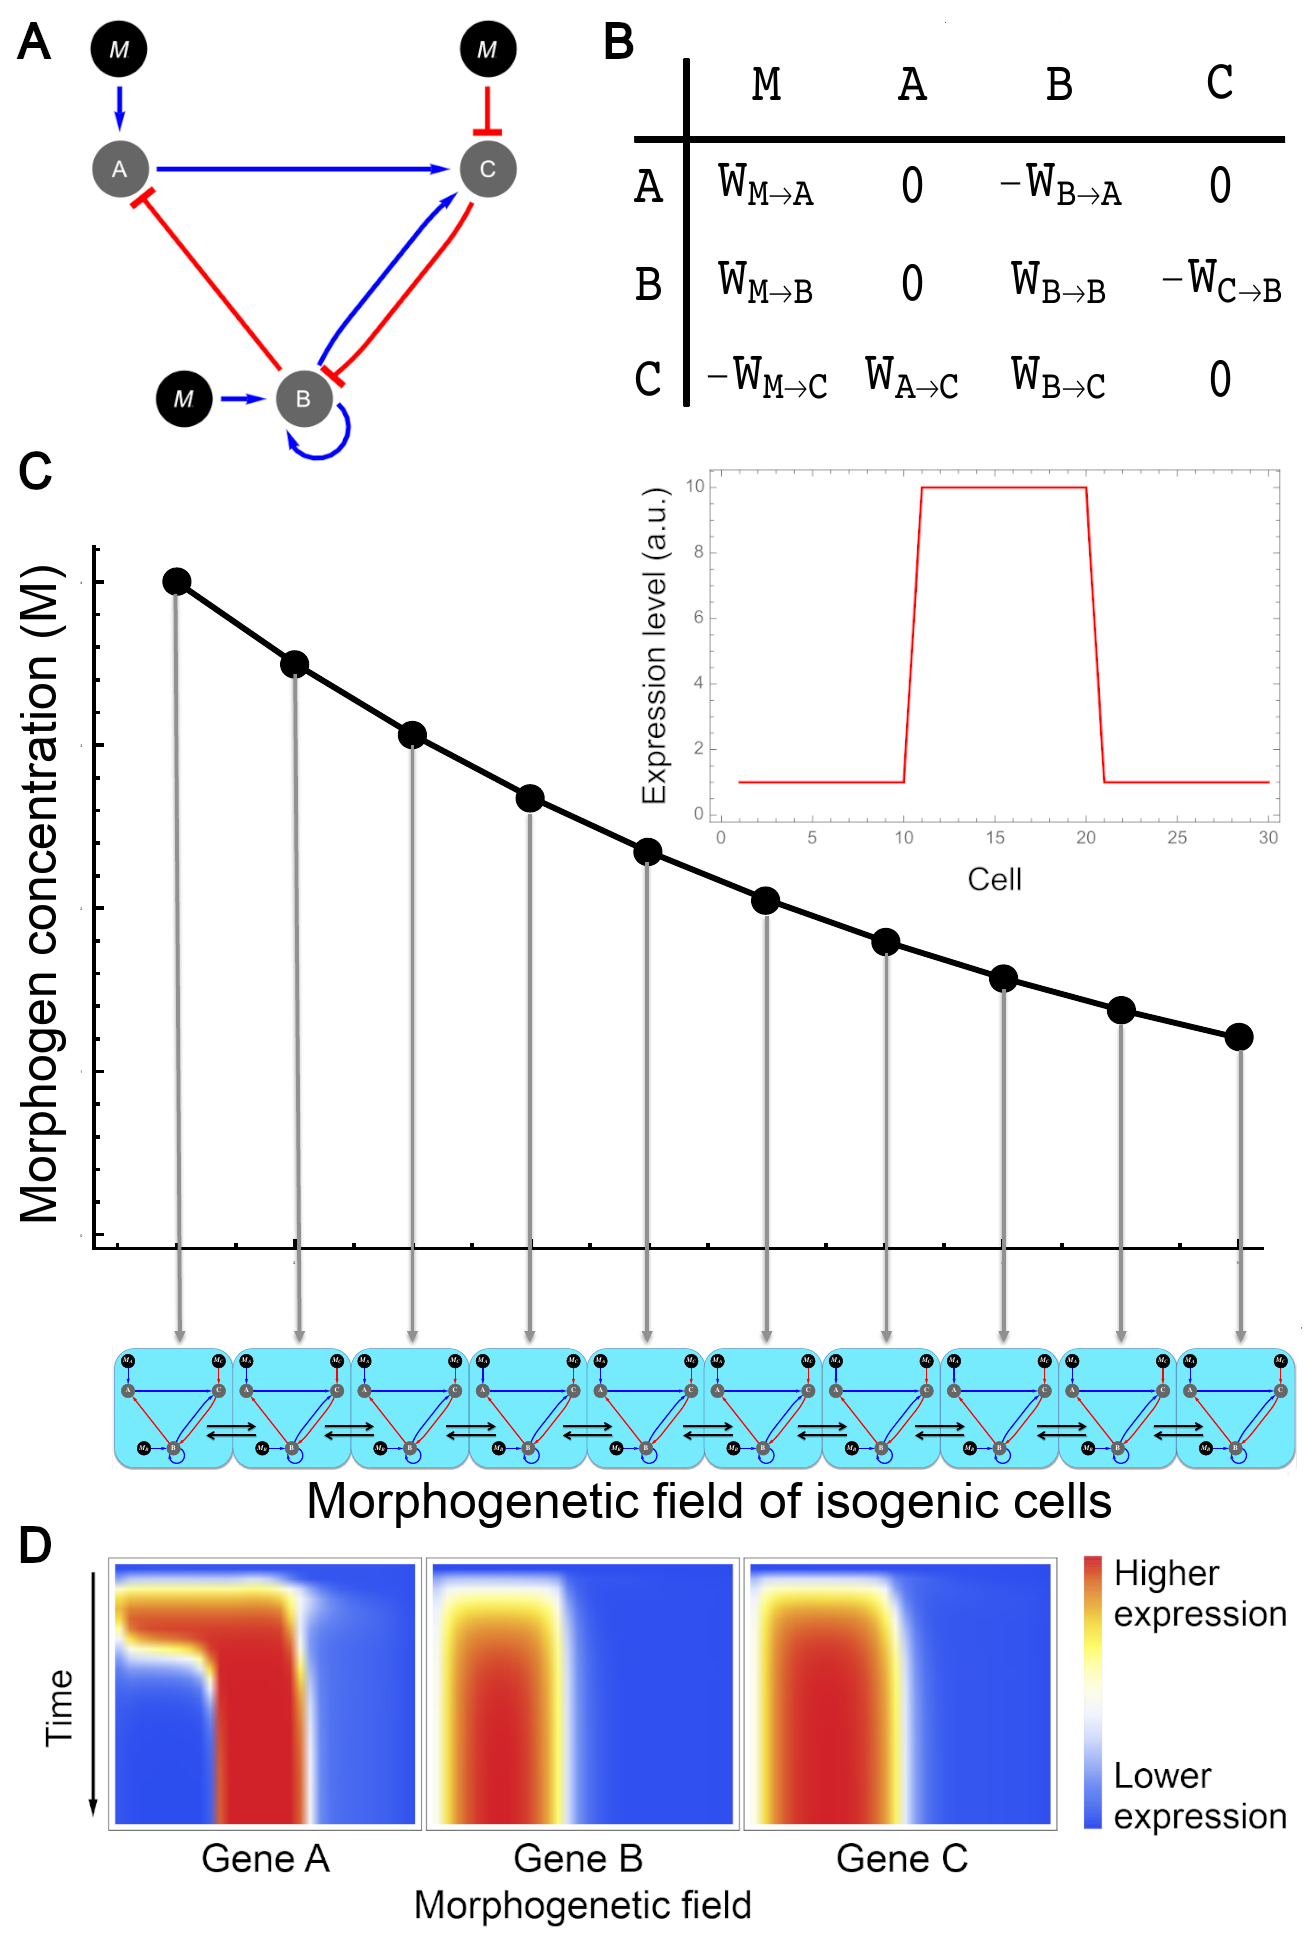
\includegraphics[width=\textwidth]{figures/metodos/Fig1}
    \caption{\bf Modelling of GRNs.}
    (A) GRN represented as a directed graph with activation (blue arrows) and
    inhibition (red arrows) interactions. Black circles
    tagged with a \textbf{M} represent the morphogen; \textbf{A}, \textbf{B} and
    \textbf{C} represent genes in the network.
    (B) The same GRN represented as an adjacency matrix in which positive values
    represent activation, negative ones represent inhibition and
    zeros represent no interaction.
    (C) Morphogenetic field. In our model the field was composed of a linear
    array of 30 isogenic cells and a morphogen gradient concentration described
    by an exponential decay function. Horizontal arrows between cells represent
    diffusion of gene products between adjacent cells. Optimal gene expression
    pattern is shown top right.
    (D) Heatmap of spatiotemporal expression profile of a GRN where blue
    colors represent lower expression and red colors represent higher
    expression.
 \label{fig:model}
\end{figure}

In our model the morphogen could interact with any of the three genes on the
GRN, but could not be affected by them. The morphogenetic field was defined by
an unidimensional array of 30 isogenic cells exposed to the morphogen
concentration gradient (Fig~\ref{fig:model}C). The initial concentration of
each gene product in all cells was set to 0.1 in all simulations.\\

\subsection*{Mathematical model}

Our model is a modification of the model used by Cotterell \& Sharpe~\cite{Cotterell2010}
and proposed by Reinitz et al.~\cite{Reinitz1995}. The
model is a dynamical system that describes the change in concentration of gene
product \emph{i} in time, as shown in Eq~\ref{ec:modelo-gral}.

 \begin{eqnarray}
  \frac{d[G]^i_n}{dt}
  = g(u^i) + D_i \cdot [ ([G]^i_{n-1}-[G]^i_n) +([G]^i_{n+1}-[G]^i_n)]-\delta_i
  \cdot [ G ]^i_n ,
  \label{ec:modelo-gral}
 \end{eqnarray}
\noindent
in which $[G]^{i}_{n}$ is the concentration of the i-th gene in the \emph{n}-th
cell ($[G]^{i}_{n} ≥ 0$), $g(u^i)$ is a function describing the relationship
between the interactions on the \emph{i}-th gene and its expression
Eq~(\ref{ec:input-func}) and described in more detail below. $D_i$ and
$\delta_i$ are the diffusion and the degradation rate of \emph{i}-th gene
product, respectively.\\

Sigmoid functions are often used to approximate Hill functions describing gene
activation/inhibition in which steepness can be modulated by mechanisms as
molecular cooperativity and target sequestration \cite{ricci2011}. This approach
has been used extensively to model the response of signaling pathways and gene
interactions in GRNs \cite{mendoza2006, vu2007, zhang2013, armao2016}.
Moreover, differential equation models using sigmoid functions have shown to
fit gene expression data \cite{chen2005, dahlquist2015}. In this study, the
input function representing regulatory interactions is a sigmoid function
described by Eq~\ref{ec:input-func}.

\begin{equation}
 g(u^i) = \frac{1}{1 + \exp(a - b \cdot u^i)},
 \label{ec:input-func}
\end{equation}
\noindent
in which $a$ is the sigmoid steepness, equal to 5; $a/b$ is the threshold value,
set to 1 for all simulations, and $u^i$ is the following equation:
\begin{equation}
 u^i = \sum_j w_{ij} \cdot [G]^j_n + w_{im} \cdot [M]_n.
 \label{ec:mat-sum}
\end{equation}

This equation sums the interactions acting upon the \emph{i}-th gene, being
$w_{ij}$ the interaction strength of the \emph{j}-th gene upon the \emph{i}-th
gene and $w_{im}$ the interaction strength of the morphogen upon the \emph{i}-th
gene. $[G]^j_n$ and $[M]_n$ are the concentrations of the \emph{j}-th gene
product and the morphogen in the \emph{n}-th cell.

\subsection*{Morphogen spatial distribution}

The morphogen concentration along the morphogenetic field is described by
Eq~\ref{ec:morph}.
\begin{equation}
 M = A_0 \cdot \exp(-c/h),
 \label{ec:morph}
\end{equation}
\noindent
were $A_0$ is the concentration of the morphogen in the position zero of the
morphogenetic field and was set to 1 in our experiments; $c$ is the cell index,
defined as the ratio between the \emph{n}-th cell from left to right and the
total number of cells, and $h$ is a decay parameter, whose value in our model
was set to 0.4. We do not consider here how the morphogen gradient can be
formed, i.e., we do not consider morphogen dynamics but we assume a static
gradient.

The phenotype of a GRN was defined as the expression pattern of each gene along
the morphogenetic field after 500 time steps of integration of the dynamical
system. We chose that number of time steps because numerical experiments showed
that GRNs reached the steady state in approximately 300 steps (\nameref{S1_Fig}).

\subsection*{Optimal pattern definition}

The optimal pattern of gene expression defined in this study consists in cells at
the border of the field ($n<11$ and $n>20$) displaying expression levels lower than
10\% of the maximal level observed along the field of cells for the output gene,
and cells at the middle of the field ($n ∈ [11,20]$) displaying expression
levels greater than 90\% of the maximal level observed along the entire field
for the output gene (Fig~\ref{fig:model}C).

\subsection*{Search space algorithm}

The Markov chain Monte Carlo (MCMC)-like algorithm used to produce the set of
gene regulatory networks (GRNs) consisted in the following steps:

\begin{enumerate}
 \item{\bf Generate a random GRN.}

 \item{\bf Numerically solve the dynamical system for the GRN from t=0 until
 t=500.} We integrated the differential equation using the function NDSolve from
 Wolfram Mathematica 11 with the option “EquationSimplification” and the
 “Residual” simplification method.

 \item{\bf Evaluate fitness by comparing the GRN phenotype with the optimal
 phenotype (Fig~\ref{fig:model}C).} In order to compute the fitness
 function for each GRN we used three different filters. The first filter
 assesses whether the expression profile of the output node reaches a
 quasi-steady state:
 \begin{equation}
  S_{filter} = \left( \frac{1}{I \cdot N}\right) \sqrt{\sum_{i=1}^{I=3}
  \sum_{n=1}^{N=30} ([G]_n^i(t=500) - [G]^i_n(t=250))^2}.
 \end{equation}

 The expression profile was considered to have reached the steady state if
 $S_{filter} < 0.001$.\\

 The second filter measures the spatial heterogeneity in the field:
 \begin{equation}
  P_{filter} = \left( \frac{1}{I \cdot N} \right) \sqrt{ \sum_{i=3}^{I=3}
  \sum_{n=1}^{N=30} \left( [G]^i_n - \langle [G]^i_n \rangle \right)^2 },
 \end{equation}

 where $\langle [G]^i_n \rangle$ is the mean concentration of the \emph{i}-th
 gene along the field at $t=500$.\\

 The third filter relates the Manhattan Distance ($D_{obs}$) between an
 expression pattern and the optimal pattern with the maximum distance achievable
 ($D_{max}$):
 \begin{equation}
  \mathit{PF}_{eff} = 1 - \frac{D_{obs}}{D_{max}}.
 \end{equation}

 In this function, the expression profile of the output gene was normalized and
 discretized so that each expression value for each cell in the field was an
 integer ranging from 1 to 10.\\

 The filters mentioned above are integrated in the following functions that
 evaluate the quality of a given phenotype:

 \begin{equation}
  Q_1(P_{filter}) = \left( \frac{ {P_{filter}}^{10} }{ {P_{filter}}^{10} +
  0.1^{10} } \right),
 \end{equation}
 \begin{equation}
  Q_2(S_{filter}) = \left( \frac{ 0.1^2 }{ {S_{filter}}^2 + 0.1^2 } \right).
 \end{equation}

 Finally, these quality functions were used to compute the fitness score with
 the following fitness function:
 \begin{equation}
  F = \mathit{PF_{eff}} \cdot Q_1(P_{filter}) \cdot Q_2(S_{filter}).
 \end{equation}

 \item {\bf Mutate GRNs randomly and evaluate fitness again.} Mutations
included changes in the  numerical values of degradation and diffusion
parameters and interaction strengths, and addition and removal of interactions
among genes and between the genes and the morphogen. If fitness of the mutated
GRN was greater or equal than that of the previous GRN, mutated GRN was saved
and the cycle continued from step 2. This cycle was repeated 50000 times, and a GRN
sampled at a given step and with a fitness score ≥ 0.95 was saved to a file as
long as its associated topology had not been sampled in previous steps.

\end{enumerate}

Steps 1 to 5 were iterated 500 times, resulting in a set of 2061 GRNs with a
striped pattern of gene expression in at least one gene.

The source code for the search space algorithm and other parts of analysis is
available at \url{https://github.com/Nesper94/gene-regulatory-networks}.

\subsection*{Classification of GRNs}

In order to group all the isomorphic (i.e. topologically equivalent) networks from
the totality (2061) of sampled GRNs we used a
classification algorithm that selected a random GRN and generated all
isomorphs of that GRN by interchanging rows of the adjacency matrix
($i \leftrightarrow j$) while interchanging the corresponding columns
($i+1 \leftrightarrow j+1$). The
algorithm then compared all six isomorphs with other GRN and classified the
topologies in the same group if they were isomorphic networks.

\subsection*{Neutral network}

The neutral network was obtained by generating all possible isomorphs of a
network topology and then calculating the minimal Hamming distance between these
isomorphs and other network topologies. The Hamming distance between two
topologies was calculated using the following equation:
\begin{equation}
 D_H(W^A, W^B) = \sum_{ij} \mid sgn(w_{ij}^A) - sgn(w^B_{ij}) \mid .
\end{equation}

We adopted the same definition of neighborhood as Cotterell \&
Sharpe~\cite{Cotterell2010}, in which two topologies were neighbors if the gain or
removal of any one interaction can transform one of the topologies into the
other.

\subsection*{Robustness analysis}

In order to evaluate the robustness of the different topologies to perturbations
in parameters of interactions between genes we took a GRN belonging to each one
of the network topologies and we modified each interaction independently by
increasing and decreasing its value by 20\%. For topologies with 3 or more
GRNs we chose the most similar to the mean configuration for that topology.\\

As a measure of the robustness of the topology we chose the proportion of times
in which a perturbation resulted in a GRN with a fitness greater or equal to
0.95. Additionally, we considered a topology to be robust if the previous
measure was greater or equal to 0.5.\\

As a measure of the robustness of subgraphs (see “Classification of topologies”)
we calculated the mean of the robustness measure of all the topologies
containing a particular subgraph.\\

\subsubsection*{Robustness of topology 9 to perturbations in non-network parameters}

In order to estimate the robustness of topology 9 to changes in parameters that
control morphogen gradient and changes in initial concentrations of gene
products, we generated 100 fitness values for each one of the 19 GRNs
belonging to topology 9; in each of these 100 assays we chose $A_0$, $h$ or
initial concentrations randomly from a Normal Distribution with $\mu = 1$ for
$A_0$, $\mu = 0.4$ for $h$ and $\mu = 0.1$ for initial concentrations and a
Coefficient of Variation of 30\% in each case.

\subsection*{Shannon entropy}

We calculated the Shannon entropy Eq~(\ref{ec:shannon}) of the network
topologies abundance distribution in order to test if this distribution could be obtained
by chance with a probability greater than 0.05. In order to obtain a 95\%
confidence interval, we generated 30 samples of a set of 2061 random matrices
and calculated the Shannon entropy in bits for each sample and tested these data
for normality.
\begin{equation}
 H = -\sum p(x) \cdot \log_{2}p(x).
 \label{ec:shannon}
\end{equation}

\subsection*{Classification of GRNs phenotypes}

In order to classify each GRN by its spatiotemporal expression profile (its
dynamics of expression), we selected expression profiles of GRNs from time step
0 to time step 250 each 10 time steps, for a total of 26 expression profiles
over time. These spatiotemporal expression profiles were represented as tensors
$S \in \mathbb{R}^{3 \times 26 \times 30}$, in which each element ($s_{itn} \geq
0$) is the expression level of the \emph{i}-th gene at time $t$ in cell $n$.\\

Next, we calculated the distance between all the pairs of tensors and performed
a Neighbor Joining clustering using the package Scikit Bio 0.5.5 from
Python 3~\cite{skbio2020}.

\subsection*{Classification of topologies}

In order to classify each topology by its subgraph composition, we first created
a matrix  $T = (t_{ij})$ with each row corresponding to a different topology
and 17 columns corresponding to subgraphs shown in \nameref{S2_Fig}.
Each element $t_{ij}$ of
the matrix was 1 if the \emph{j}-th subgraph was present in the \emph{i}-th
topology or 0 if the subgraph was not present.\\

With this matrix we then calculated a distance matrix in which each element
consisted in the Hamming distance between the row vectors in matrix $T$ between
each pair of topologies. We then clustered the topologies based on the
Neighbor Joining method, as implemented in the Scikit Bio
package~\cite{skbio2020}.

\subsection*{Complexity index and network descriptors}

As a measure of network complexity, we used the complexity index based on
Shannon entropy proposed by Bonchev \& Rovray~\cite{D.2005}. We calculated this
index using the following equation:
\begin{equation}
 I_{vd} = \sum_{i=1}^V a_i \cdot \log_{2} a_i,
\end{equation}
\noindent
where $a_i$ denotes the degree of the \emph{i}-th node and $V$ the number of
nodes in the network. Both the network descriptors and Pearson’s chi-square
goodness of fit tests were performed for the node degree distribution using
the built-in functions from the Wolfram Mathematica software.\\

\subsection*{Pattern formation under varying size of the morphogenetic field}
We evaluated the ability of each of the sampled GRNs to generate a striped
pattern of gene expression under varying sizes of the morphogenetic field.
Specifically, we calculated the fitness of each GRN across morphogenetic fields
composed of 10, 20, 40, and 50 cells. In these simulations we redefined the
morphogen gradient in such a way that the initial and final concentration were
constant in all the fields (\nameref{S3_Fig}A). In order to know if topologies
with the same topology had a similar fitness in the different fields, we performed
a Principal Component Analysis in Scikit-learn~0.24.2~\cite{sklearn} using the
fitness values of each in the four different fields (see \nameref{S3_Fig}).

% For placing video, \nameref{S1_Video} vel sagittis arcu lobortis.

% Place figure captions after the first paragraph in which they are cited.
% \begin{figure}[!h]
% \caption{{\bf Bold the figure title.}
% Figure caption text here, please use this space for the figure panel descriptions instead of using subfigure commands. A: Lorem ipsum dolor sit amet. B: Consectetur adipiscing elit.}
% \label{fig1}
% \end{figure}

% Results and Discussion can be combined.
\section*{Results}

The classification of GRNs showed that our initial set of 2061 GRNs can be
grouped into 714 distinct network topology classes, with each containing a
variable number of GRNs (Fig~\ref{fig:distopol}). This abundances
distribution was not produced by chance (Shannon entropy = 8.52963, 95\%
confidence interval = [10.8915, 10.9275]), and instead it displays some level
of structure, indicating the existence of network motifs.

\begin{figure}[!h]
 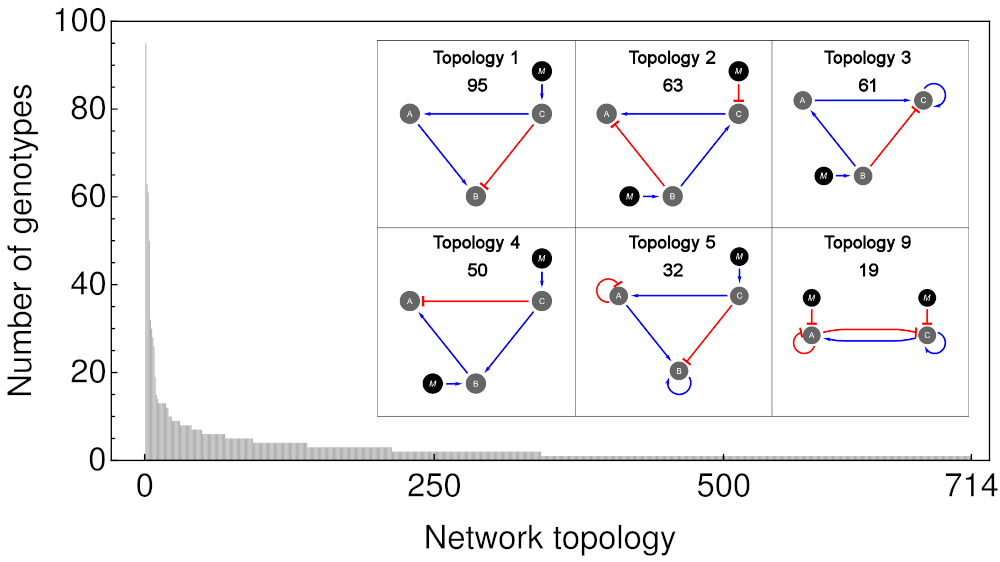
\includegraphics[width=\textwidth]{figures/results/Fig2}
 \caption{\bf Distribution of abundances of network topologies.}
 Some of the most frequent network topologies shown in the grid
 contain the I3-FFL network motif (shown on the left). In this network
 motif the gene B is activated in an indirect way by the morphogen through
 the activation of A (positive interactions), and at the same time, it
 is inactivated in a direct way by the morphogen (negative interaction).
 Topologies are numbered in order of decreasing abundance, being the
 Topology 1 the most abundant with a number of 95 genotypes. The number of
 genotypes belonging to each network topology is presented below
 topology number.
 Note that network topology number 9 produces the striped phenotype using a
 two-node GRN.
 \label{fig:distopol}
\end{figure}

The most abundant network topologies are shown in Fig~\ref{fig:distopol}.
Interestingly, among the 15 most abundant network topologies, eleven of them
presented the Incoherent type 3 Feed-Forward Loop (I3-FFL) network motif. In
addition, we found that topology number 9 could produce the striped phenotype
with only two nodes.

The neutral network (a metagraph in which each node is a network topology)
shows that most of the network topologies are grouped into a connected graph.
This graph is composed of 639 nodes that are accessible by one mutational step.
The 15 most abundant network topologies, with the exception of
number 10, are part of this graph (Fig~\ref{fig:neutral-network}). We also
found nodes inside the neutral network that had more connections between them
than with other nodes, which leads to further clustering of nodes. Interestingly in
almost every cluster one can find one or more of the 15 most abundant network
topologies. In addition, we found that the first eight most abundant network
topologies were located in the largest cluster.

\begin{figure}[!h]
 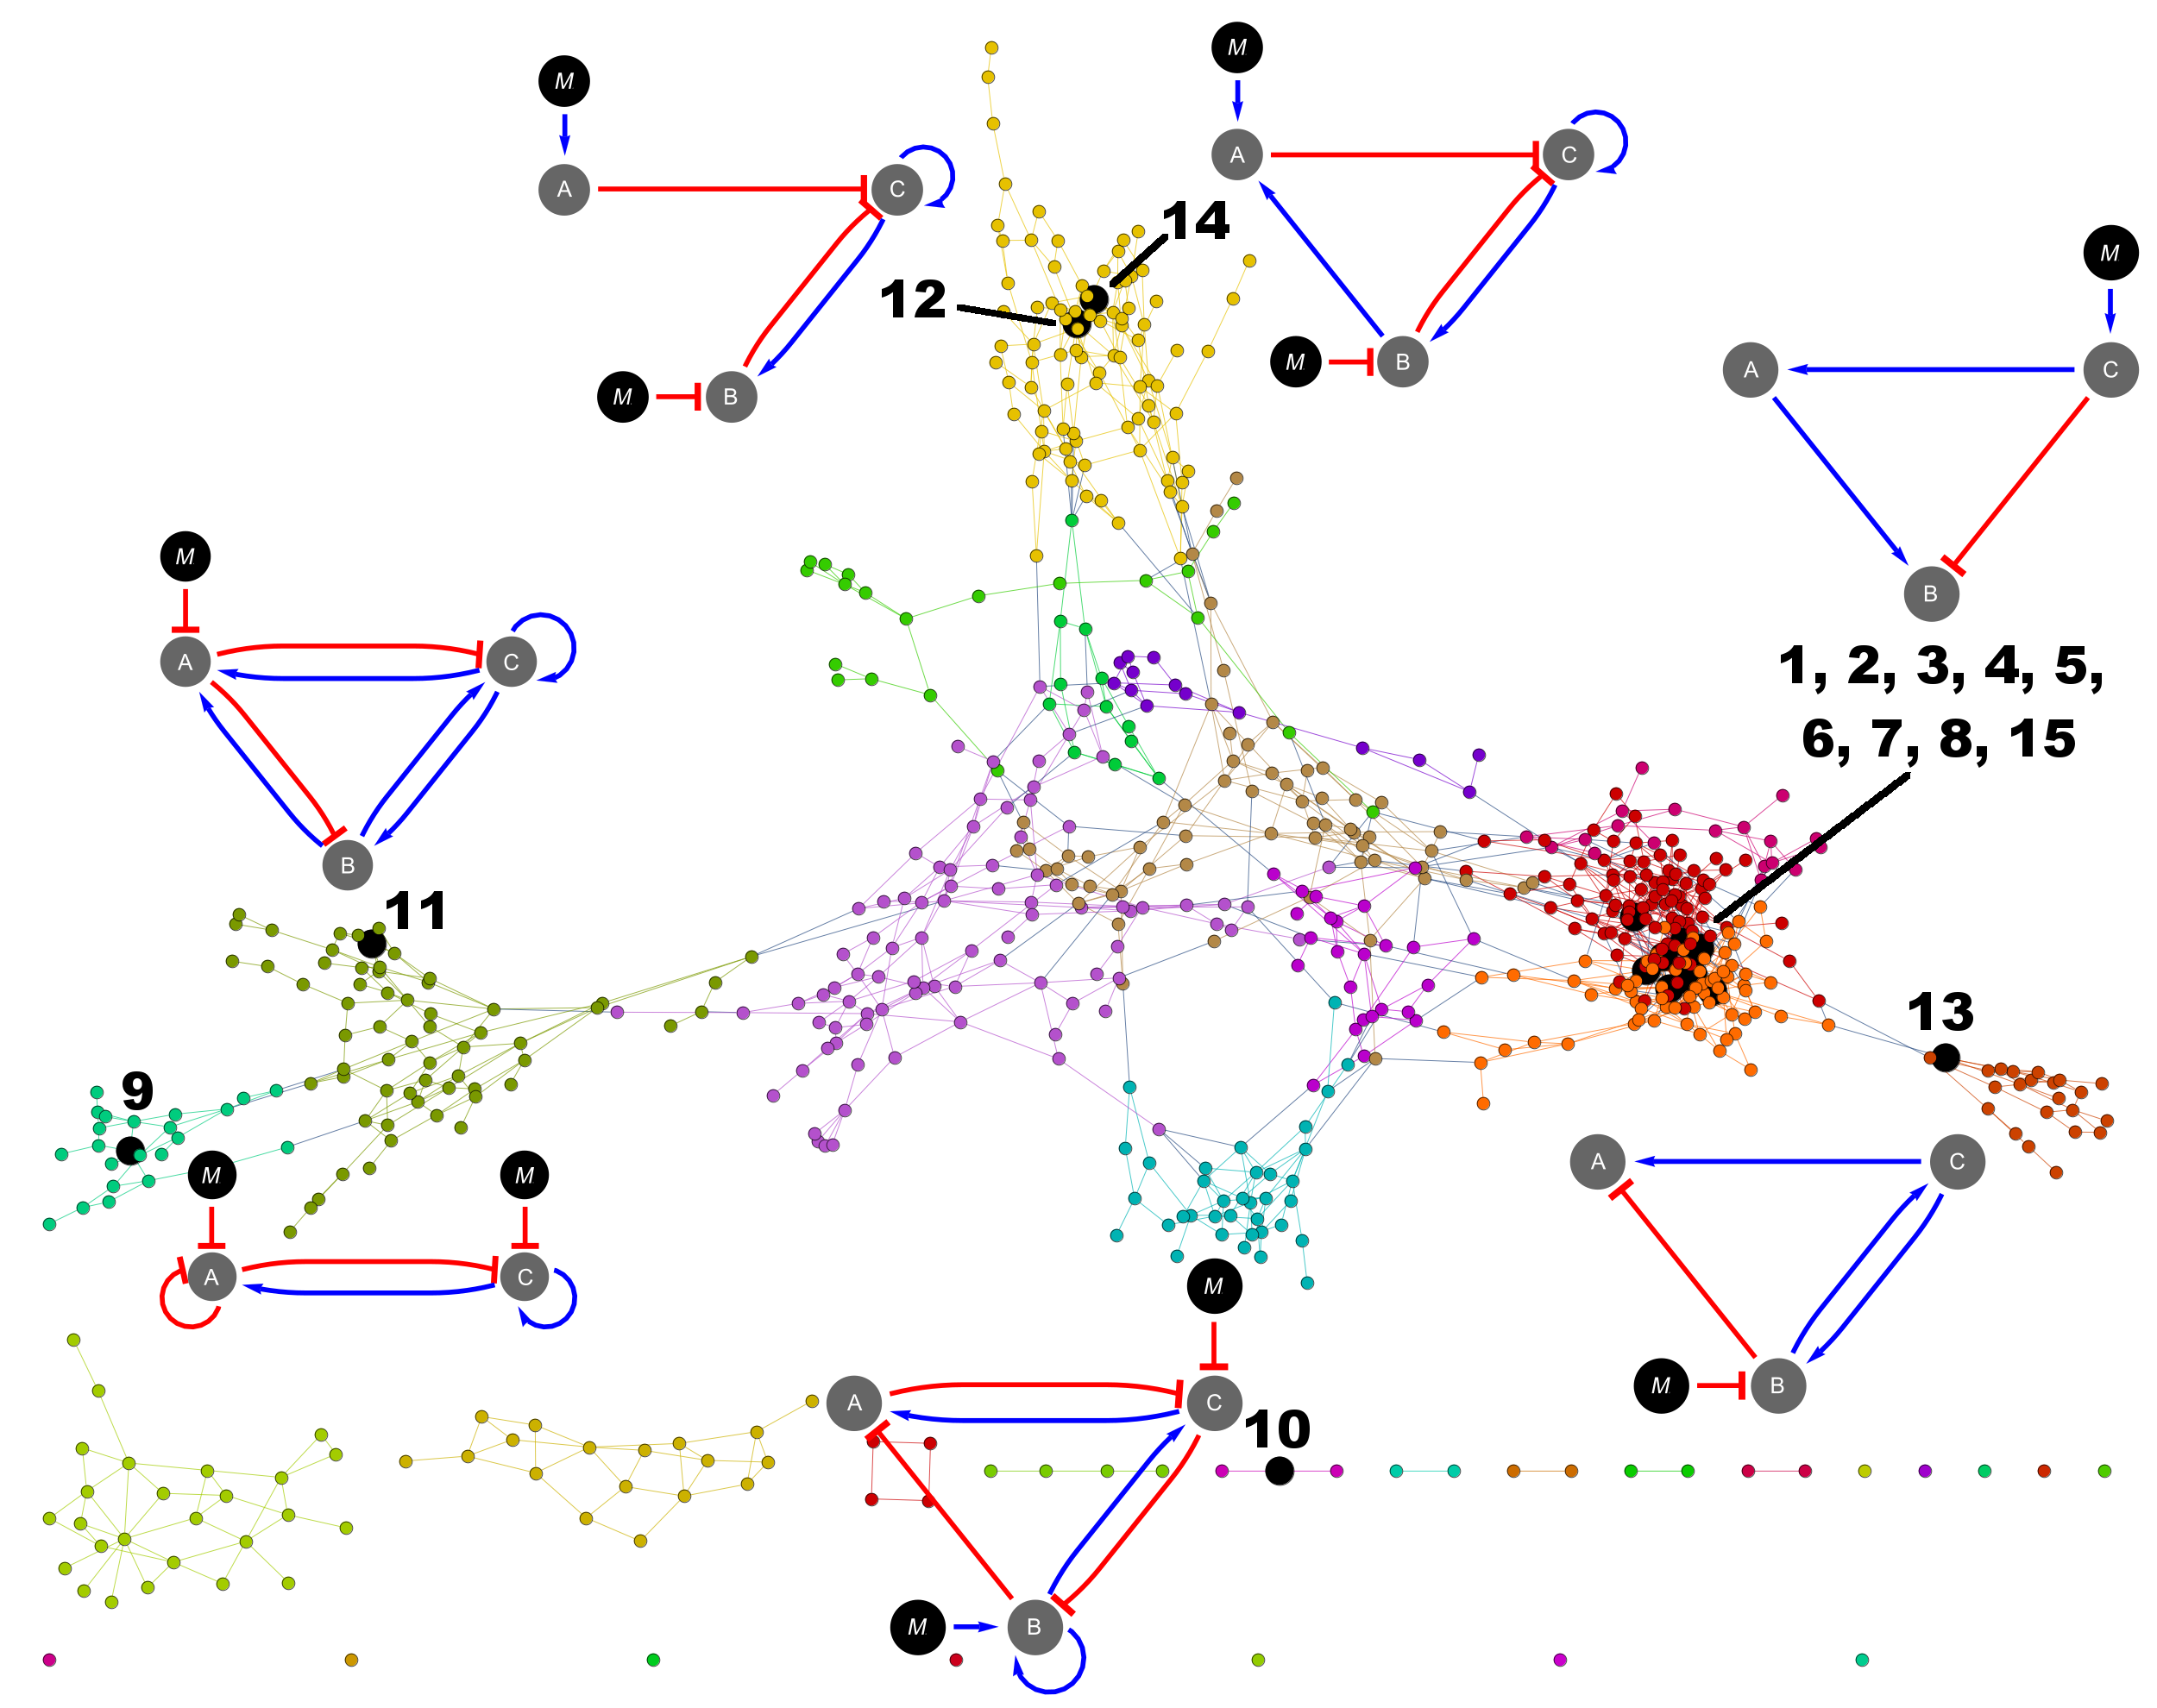
\includegraphics[width=\textwidth]{figures/results/Fig3}
 \caption{\bf Neutral network.}
 This graph shows network topologies connected by one mutational step, where
 each node represents a single topology. Black nodes represent the most
 abundant topologies. All nodes with the same
 color belong to a cluster of nodes more connected between them than with other
 nodes in the graph. The most abundant topologies are represented as
 directed graphs in the same way as in Fig~\ref{fig:model}A, except for
 the topologies 1 to 8 and 15 (orange and red clusters), in which only
 topology 1 is depicted.
 \label{fig:neutral-network}
\end{figure}

The degree distribution of this network seems to follow a Poisson distribution
(Pearson’s $\chi^2 = 12.8902$, $\text{p-value} = 0.115684$) characteristic of a
Erdös-Rényi network with many nodes and edges~\cite{Erdos1959}. This kind of
network presents a great
number of nodes with low degree and a few nodes with high degree
(Fig~\ref{fig:deg-dist}A). Nodes corresponding to topologies number one and
three showed the highest degree ($deg(1) = deg (3) = 14$). Curiously, we found
that nodes with higher degree turned out to be also those network topologies
with higher abundance
(Fig~\ref{fig:deg-dist}B). This relationship between abundance and node degree
was corroborated by the Spearman's rank correlation coefficient
($r_S = 0.353752$, $p = 6.2933\times10^{-23} $).

\begin{figure}[!h]
 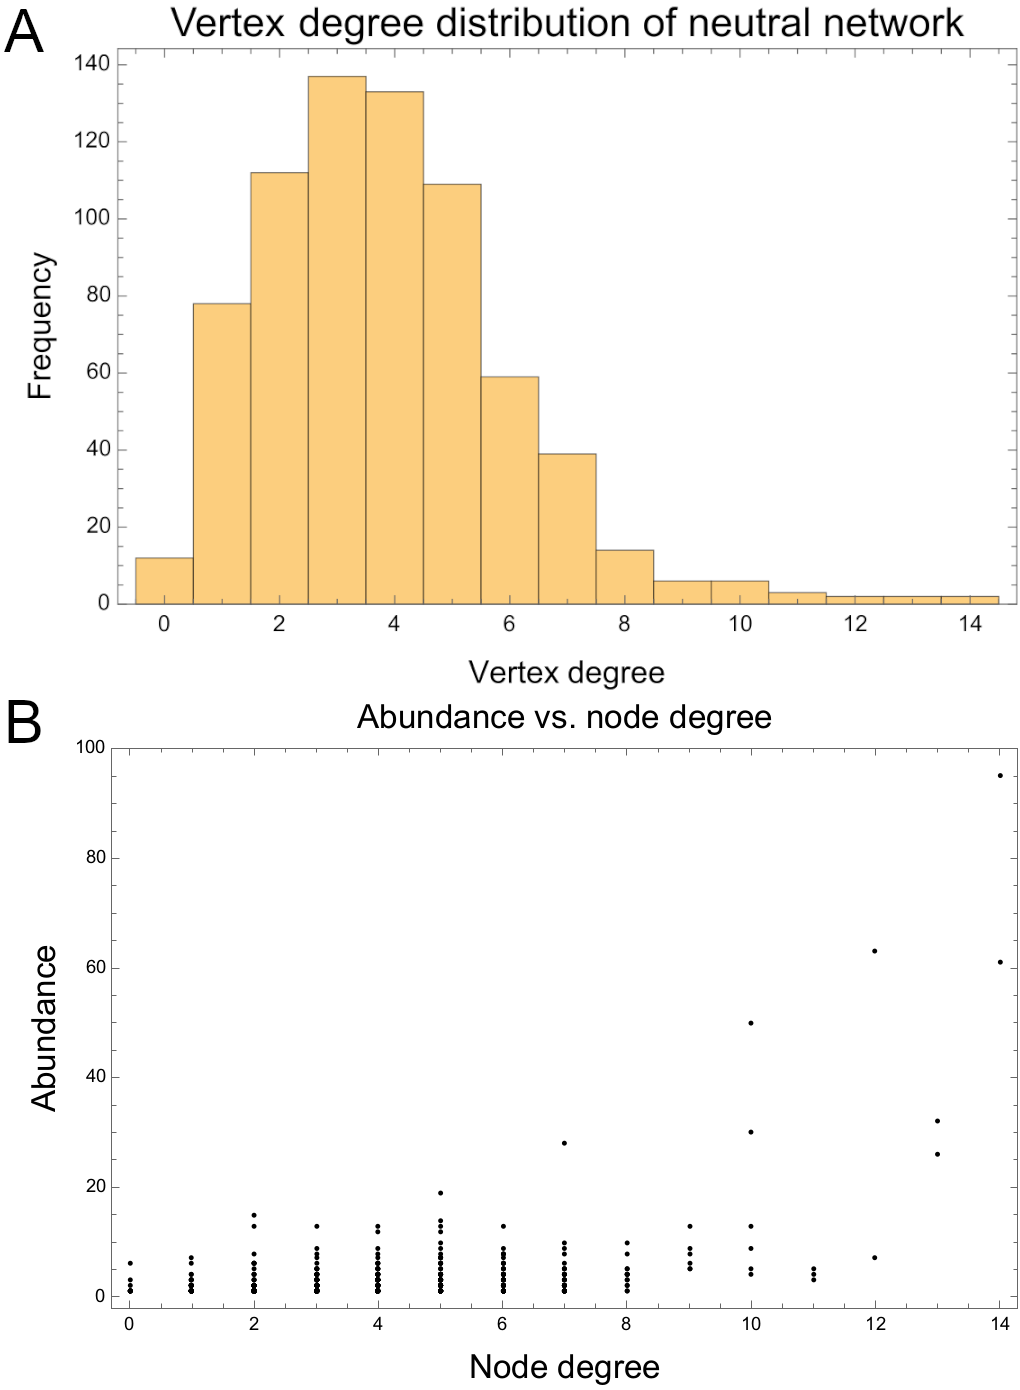
\includegraphics[width=\textwidth]{figures/results/Fig4}
 \caption{\bf Node degree in the neutral network.}
 (A) Histogram of vertex degree distribution in the neutral network.
 (B) Scatter plot of Topology abundance vs. Node degree in the neutral
 network.
 \label{fig:deg-dist}
\end{figure}

Furthermore, we examined the extent to which the metagraph of topologies
remained highly connected when joining neighbors at two mutational steps.
Interestingly, we found that only topology number 420 remained isolated from
the rest of topologies in the metagraph (Fig~\ref{fig:2neut-net}).

\begin{figure}
 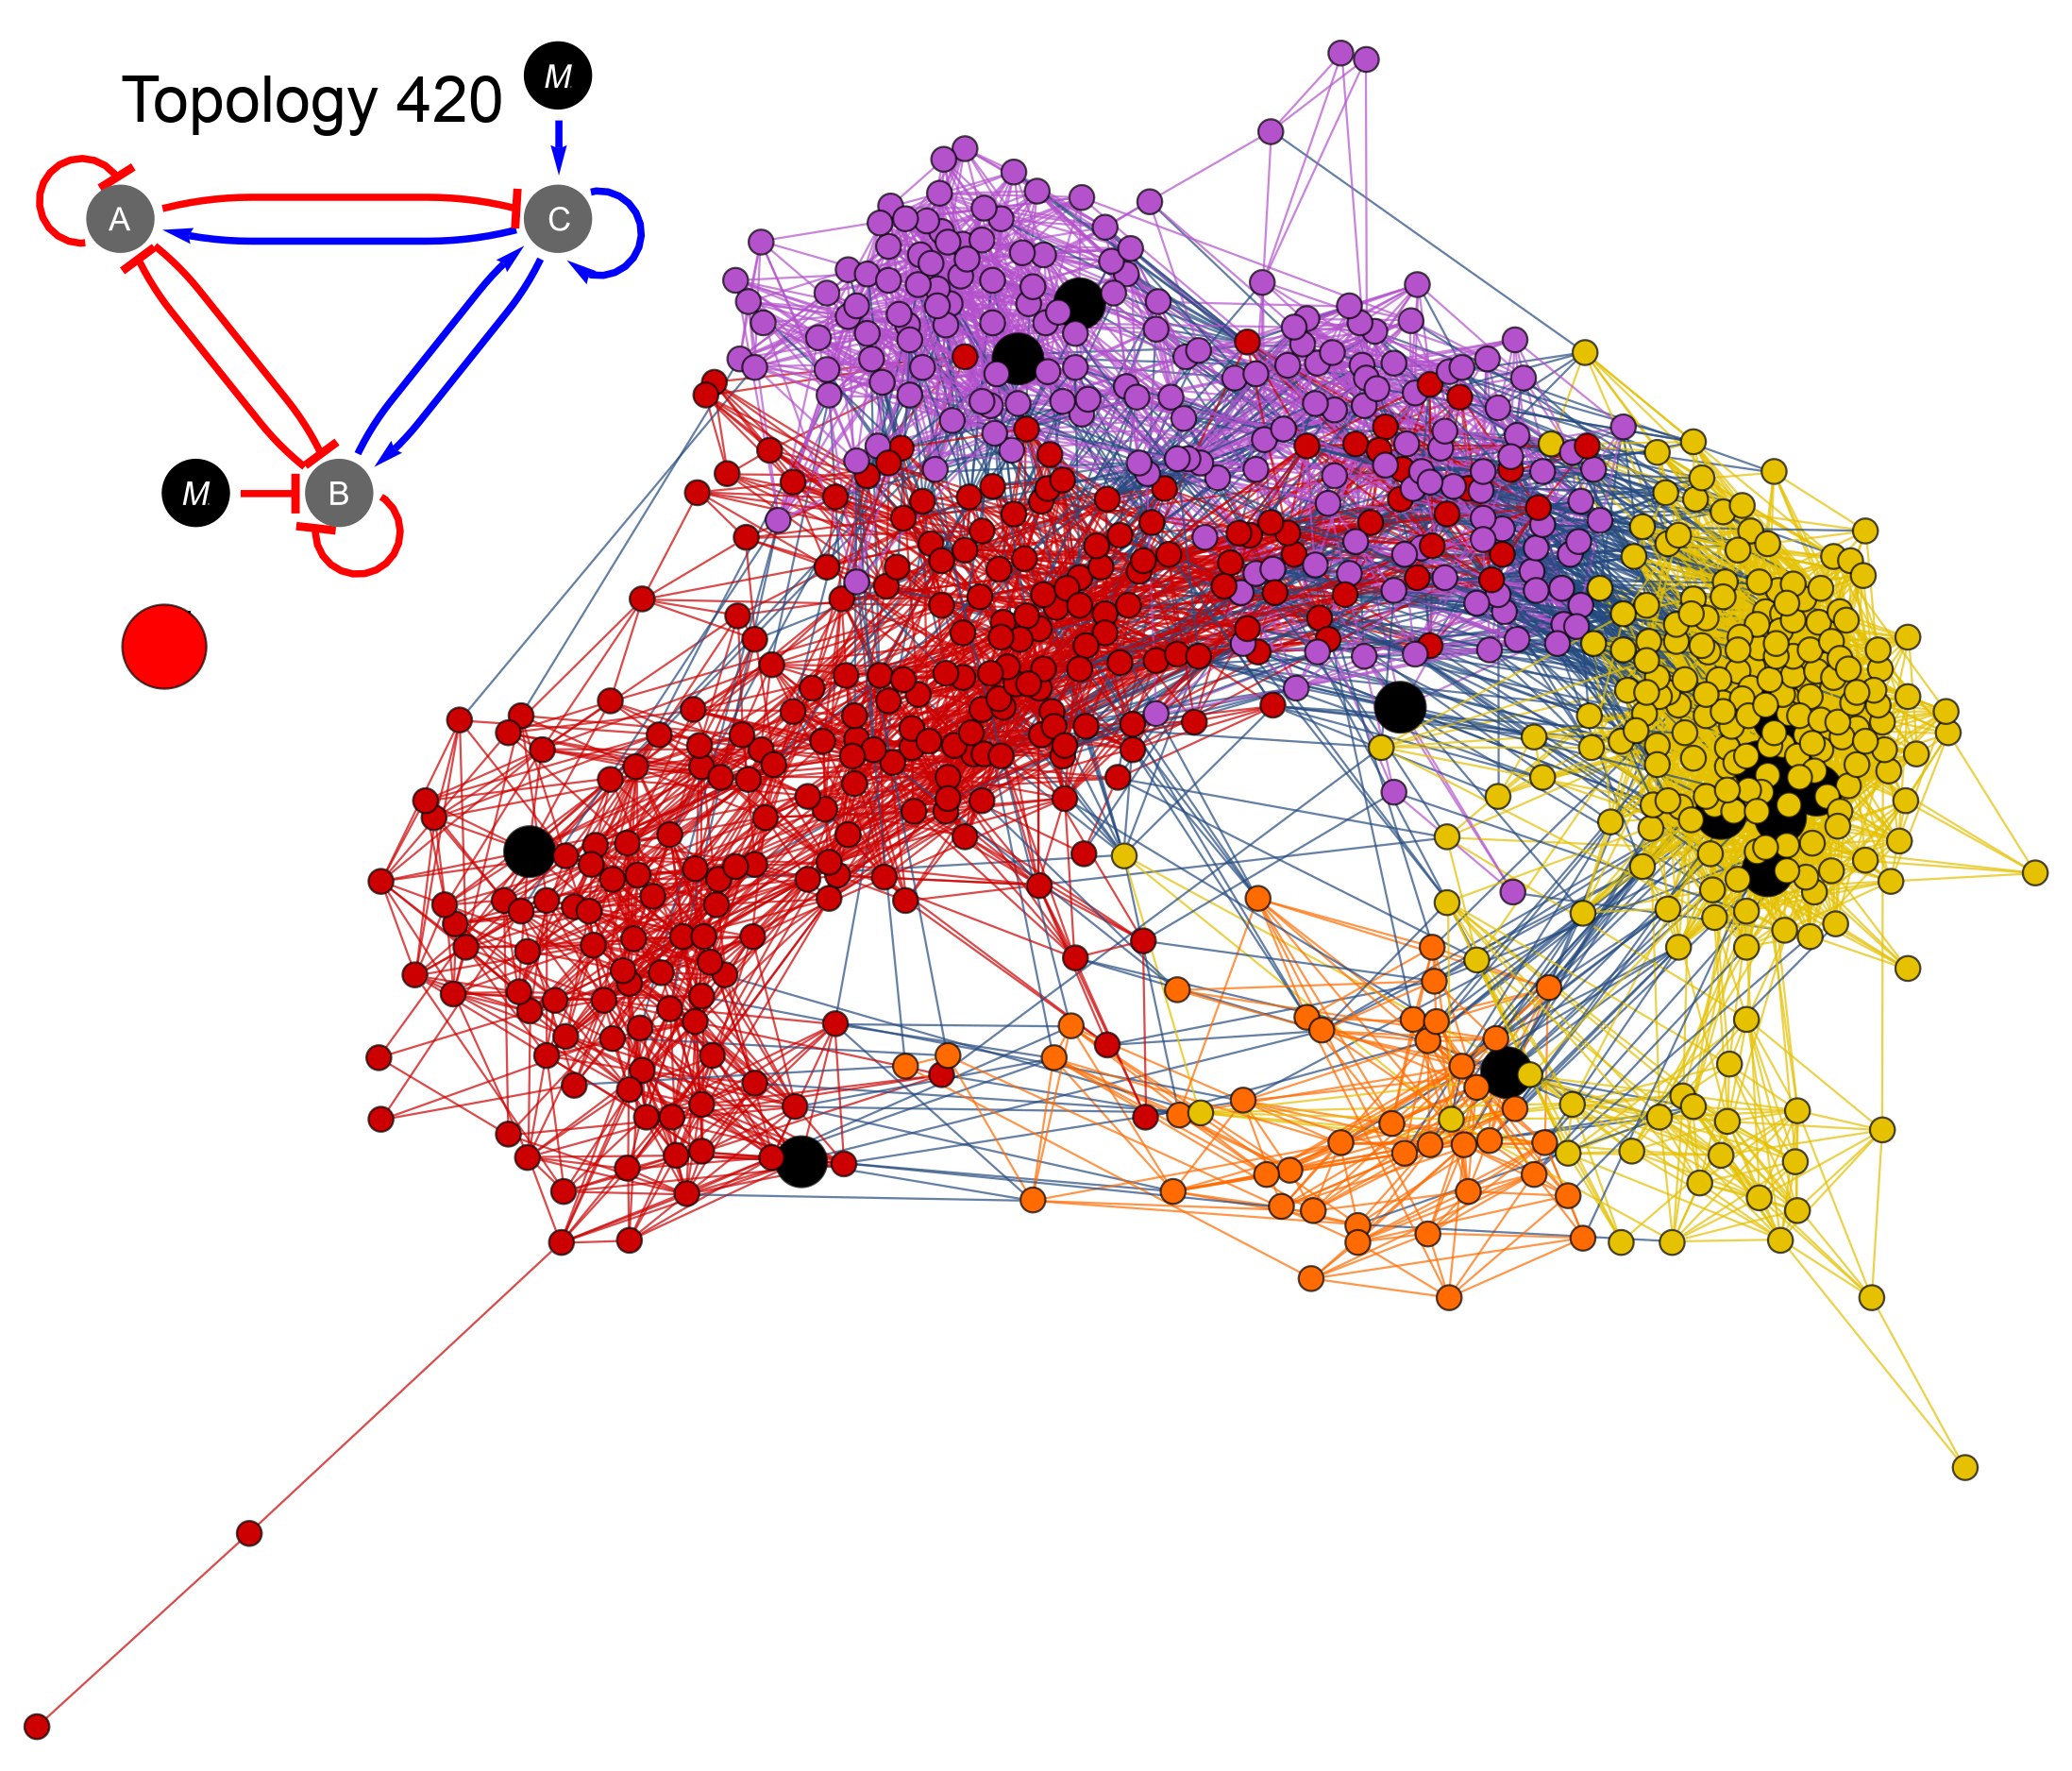
\includegraphics[width=\textwidth]{figures/results/Fig5}
 \caption{\bf Network of topologies separated by two mutational steps.}
 The network shows that almost all the topologies are connected by two or less
 mutational steps. Big red circle represents topology 420 that remains
 unconnected from the main graph. Big black circles correspond to the 15
 most abundant topologies described in Fig~\ref{fig:neutral-network}.
 Different colors in the graph represent different clusters of topologies.
 \label{fig:2neut-net}
\end{figure}

Next to topological robustness, we investigated the robustness of the sampled
network topologies to parameter changes (see Methods). Fig~\ref{fig:ab-rob}A
illustrates the association between the abundance of a topology class versus its
robustness. We did not find a significant correlation between
these two variables ($r_S = −0.0389724$, $\text{p-value} = 0.298475$).
However, when we grouped those topologies containing
the same subgraph and calculated their mean robustness, we found that between
the most robust subgraphs is the ``Bistable'' motif, the I3-FFL, as well as
the ``Overlapping domains'' motif (which is a variation of the I3-FFL), which
have been previously reported in Cotterell \& Sharpe~\cite{Cotterell2010}
(see \nameref{S2_Fig} and \nameref{S1_Table}).

\begin{figure}[!h]
 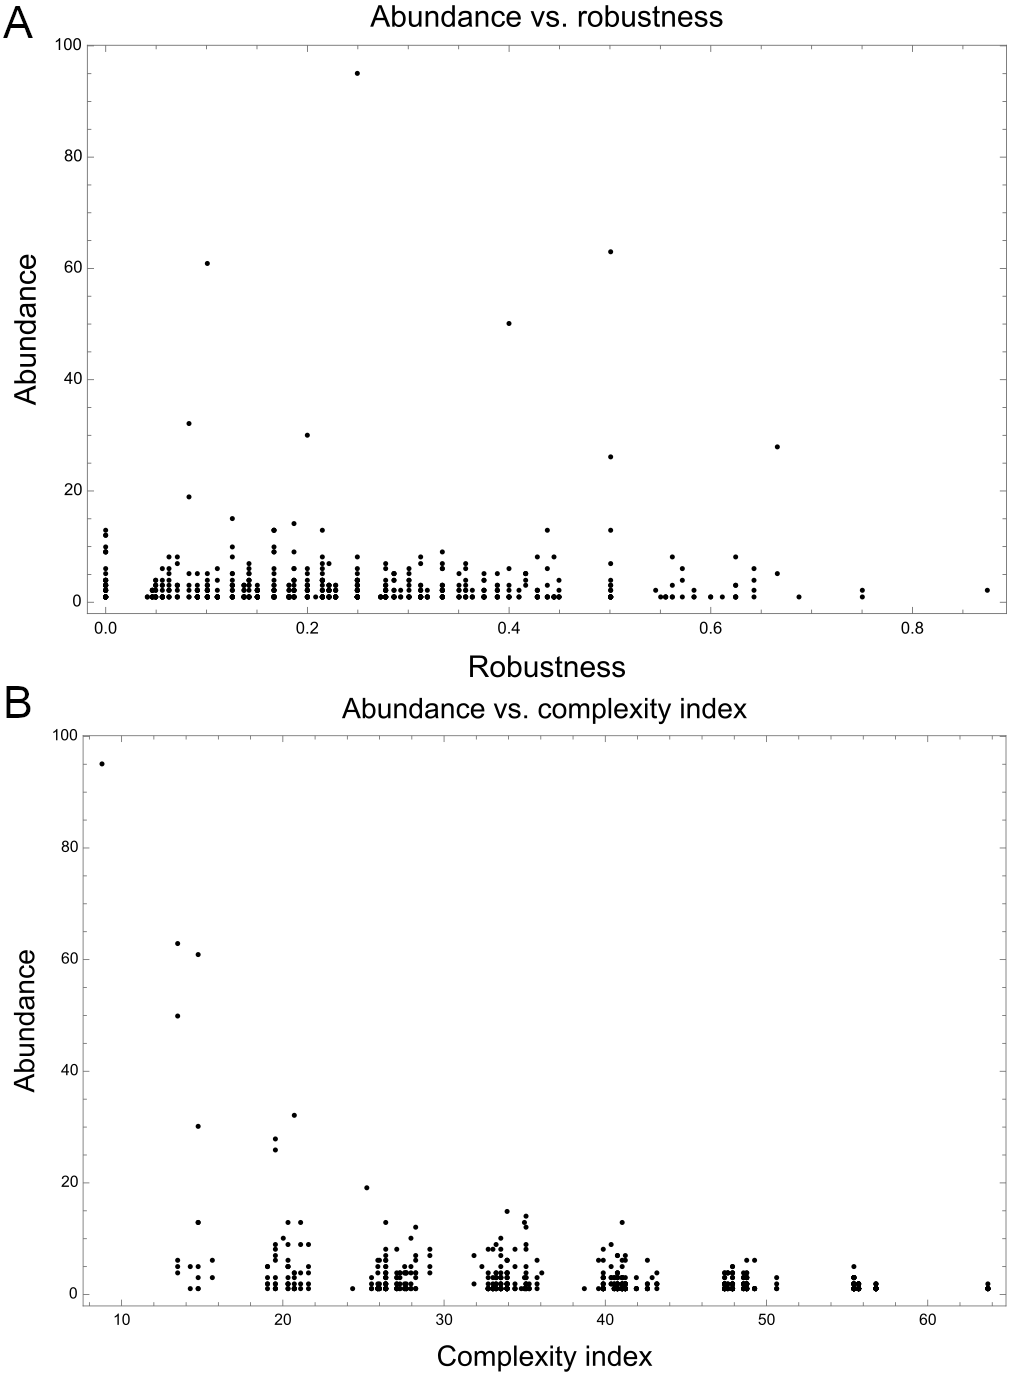
\includegraphics[width=\textwidth]{figures/results/Fig6}
 \caption{\bf Relationship between Abundance and robustness and complexity
 index.} (A) Abundance vs. Robustness. The robustness of each topology was
 calculated as the ratio of perturbations in which the fitness was greater or
 equal to 0.95 with respect to the total of perturbations performed.
 (B) Abundance vs. Complexity index. Each point in the plot represents one of
 the 714 network topologies. More complex topologies tend to be less abundant
 than simple topologies
 ($r_S = -0.316653$, $\text{p-value} = 2.25161\times10^{-18}$).
 \label{fig:ab-rob}
\end{figure}

On the other hand, analysis of the average vertex degree seems to be indicative
that network topologies are likely to withstand numerous topological
modifications (approximately 4) without significant loss in their ability to
generate a striped pattern of gene expression, representing a high fitness
solution to the prescribed task. The average complexity index of network
topologies was 39.2435 ($\pm 11.6768$) and was found to be negatively
correlated with the abundance ($r_S = -0.316653$, $\text{p-value} =
2.25161\times10^{-18}$) (Fig~\ref{fig:ab-rob}B).
Additionally, the average path length seems
to suggest that the evolutionary landscape could be easily traversed by
most network topologies without incurring in significant fitness loss as long
as mutational changes results in moves between adjacent neighbors across
the metagraph (Table~\ref{table1}). It is interesting to note that,
although the examined GRNs seem to exhibit, on average, a high robustness to
topological/parameter changes, they generally show a rather high sensitivity to
variation in the size of the morphogenetic field. For instance, we found that
when the size of the morphogenetic field was fixed at 10, 20, 40 and 50 cells
only 4.66\%, 56.82\%, 56.14\% and 41.05\%, respectively, of the examined
GRNs showed a fitness greater than 0.9 (\nameref{S3_Fig}B).

\begin{table}[!ht]
% \begin{adjustwidth}{-2.25in}{0in} % Comment out/remove adjustwidth environment if table fits in text column.
 \centering
 \caption{{\bf Network descriptors of neutral network of topologies.}}
 \begin{tabular}{|l|l|}
 \hline
 {\bf Network descriptor} & {\bf Value}\\ \thickhline
 Average vertex degree  & 3.85714 \\ \hline
 Clustering coefficient~\cite{Watts1998} & 0.117097 \\ \hline
 Average path length    & 7.25261       \\ \hline
 Graph connectedness    & 0.00540974    \\ \hline
 Graph diameter*        & 25            \\ \hline
 Average path length*   & 9.0499        \\ \hline
 \end{tabular}
 \begin{flushleft} *These descriptors were calculated for the main connected
 subgraph of the network.
 \end{flushleft}
 \label{table1}
% \end{adjustwidth}
 \end{table}

Hierarchical clustering of spatiotemporal expression profiles showed that GRNs
with topologies that seemed to be very different have indeed very similar
expression dynamics. We expected to find GRNs with the same topology to group
together but instead we found GRNs with different topologies grouped as close
neighbors (Fig~\ref{fig:clustering}A). Intriguingly, some GRNs displaying
very abundant network topologies were grouped together with GRNs displaying
very infrequent network topologies. This seems to indicate that additional
interactions in the networks are likely to represent alternative regulatory
mechanisms for fine tuning gene expression, instead of drastically changing
the expression mechanism, which can be seen in the expression dynamics of
networks with different topologies (\nameref{S4_Fig}). Additionally, clustering
of topologies revealed that there are six main groups of topologies in our set
of 2061 GRNs (Fig~\ref{fig:clustering}B).

\begin{figure}[!h]
 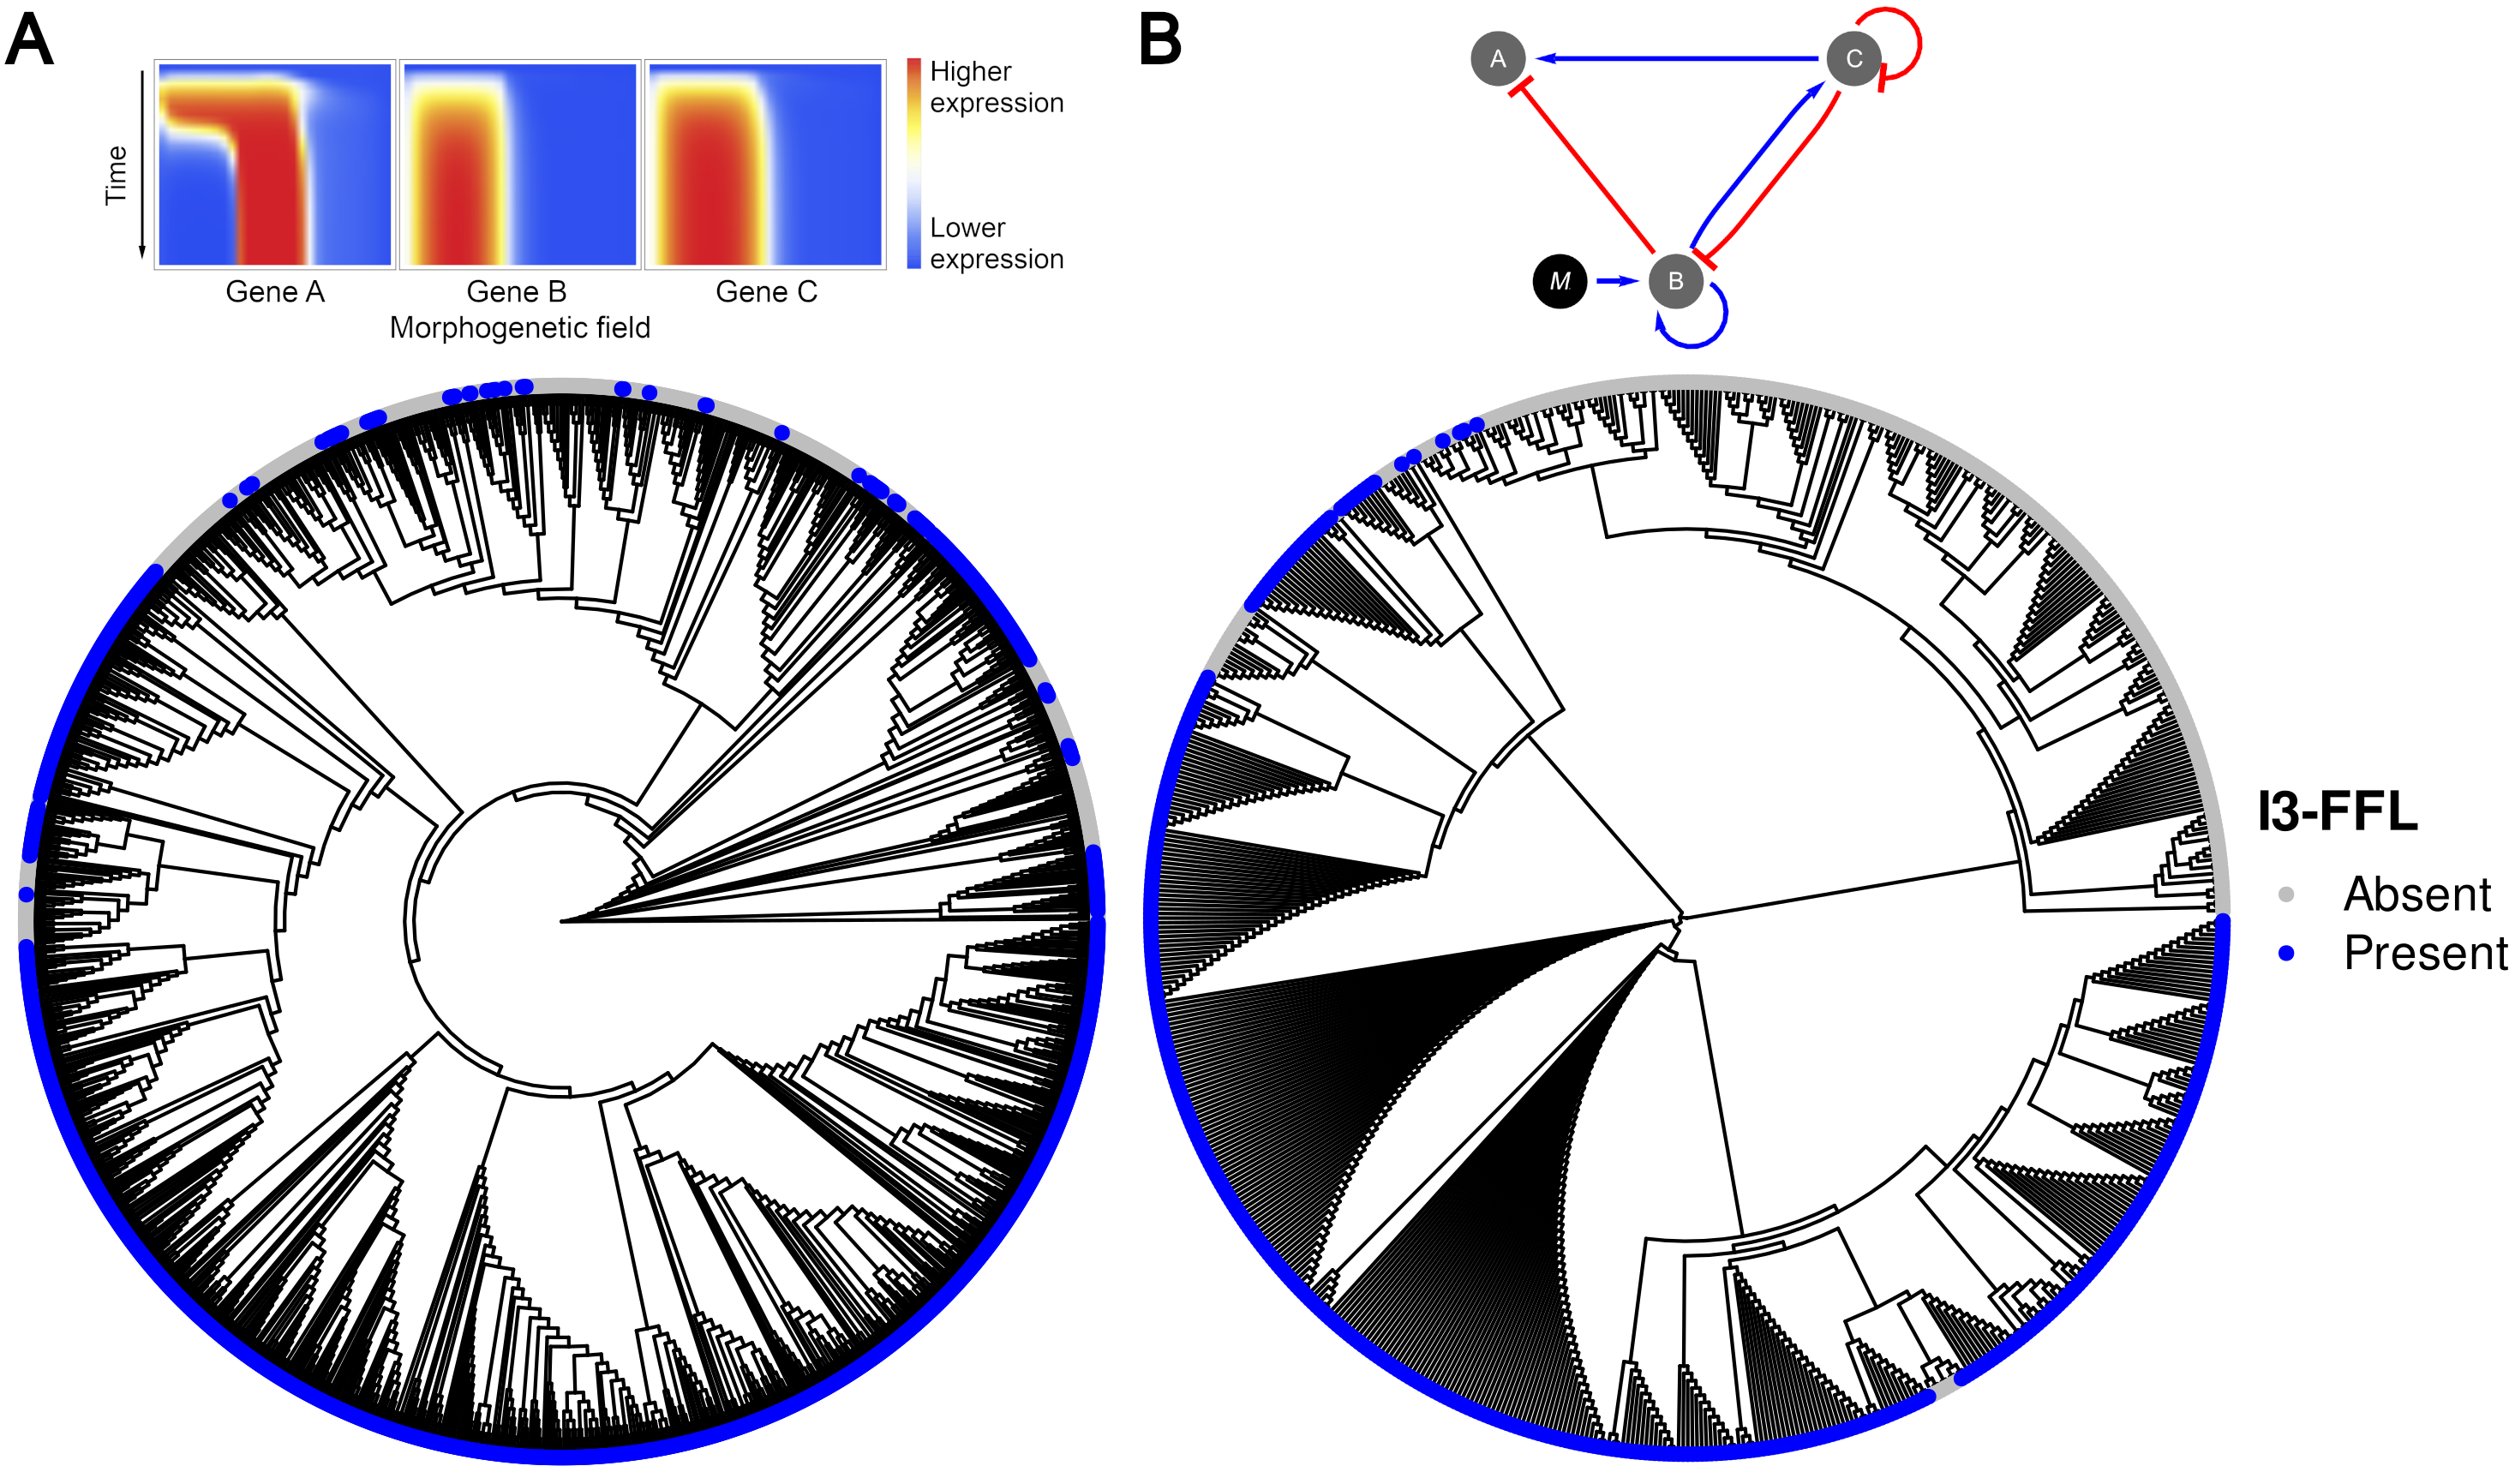
\includegraphics[width=\textwidth]{figures/results/Fig7}
 \caption{\bf Clustering of expression profiles and topologies.}
 (A) Clustering of spatiotemporal expression profiles obtained by
 neighbor joining. (B) Clustering of network topologies. Blue circles
 correspond to topologies that contain the I3-FFL network motif.
 \label{fig:clustering}
\end{figure}

Among the new network topologies we report here, perhaps one of the most
interesting ones is the topology number 9, which is able to express the striped
gene expression pattern with only two genes (Fig~\ref{fig:topol9}).
This topology is composed of a core quite similar to the Gierer-Meinhardt
mechanism~\cite{giererMeinh1972, meinhardt2000} known to generate
stripes and dots in bidimensional fields, with the only differences being
the self inhibition of gene A and the inhibition of the genes by the morphogen.
Such additional interactions in the topology number 9 play a role in restricting
the striped expression pattern to a precise location along the morphogenetic field.

\begin{figure}[!h]
 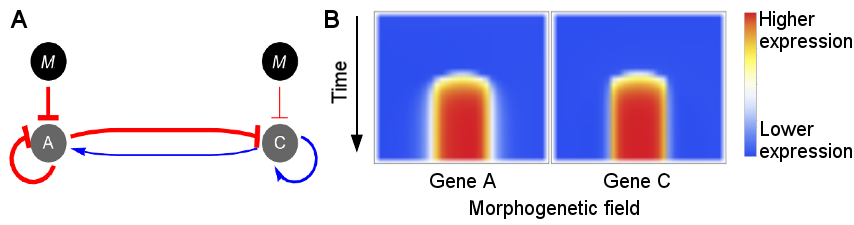
\includegraphics[width=\textwidth]{figures/results/Fig8}
 \caption{\bf Expression dynamics of topology 9.}
 (A) Network topology number 9. Although this topology consists only of two
 genes, it display a striped pattern of gene expression for both of them as
 can be observed in (B). (B) Spatiotemporal expression profile of a GRN
 with topology 9. Gene \textbf{B} is not shown as it was lost in this topology
 in the evolutionary process simulated by the search space algorithm.
 \label{fig:topol9}
\end{figure}

Despite having only two genes, the regulatory mechanism underlying
the topology 9 generates dynamically more complex expression patterns
compared to other topologies, such as the
I3-FFL; however, and despite the fact that the Gierer-Meinhardt model forms
patterns that scale with tissue size~\cite{shoaf1984}, we found that topology 9
was more sensible to changes in the morphogenetic field size than those
topologies based on I3-FFL (\nameref{S2_Table}),
indicating that the additional regulatory interactions need to be fine-tuned
depending on the number of cells in the field.\\

In the mechanism of expression of topology 9 the initial expression
pattern of gene A is uniform across the morphogenetic field, but later
on the morphogen gradient shapes its dynamics in such a way that
two important events occur: firstly, the overall expression level of the
gene A is decreased by the inhibition of the morphogen, releasing
gene C from its repression by gene A; next, gene A tend to display a
non-homogeneous spatial distribution with higher expression levels
being shifted towards the cells at the rightmost part of the morphogenetic
field.\\

These two events lead to the repression of the gene C by the gene A in the
rightmost part of the morphogenetic field and by the morphogen in the leftmost
part of the morphogenetic field, thus generating a slightly higher level of
expression of gene C in the center of the field. Because gene C activates its
own expression, a band of expression begins to form. This band of expression
then begins to activate the gene A also in the center of the field
(\nameref{S5_Fig}).
% (Fig~\ref{fig:topol9-dyn}).

% \begin{figure}[!h]
%  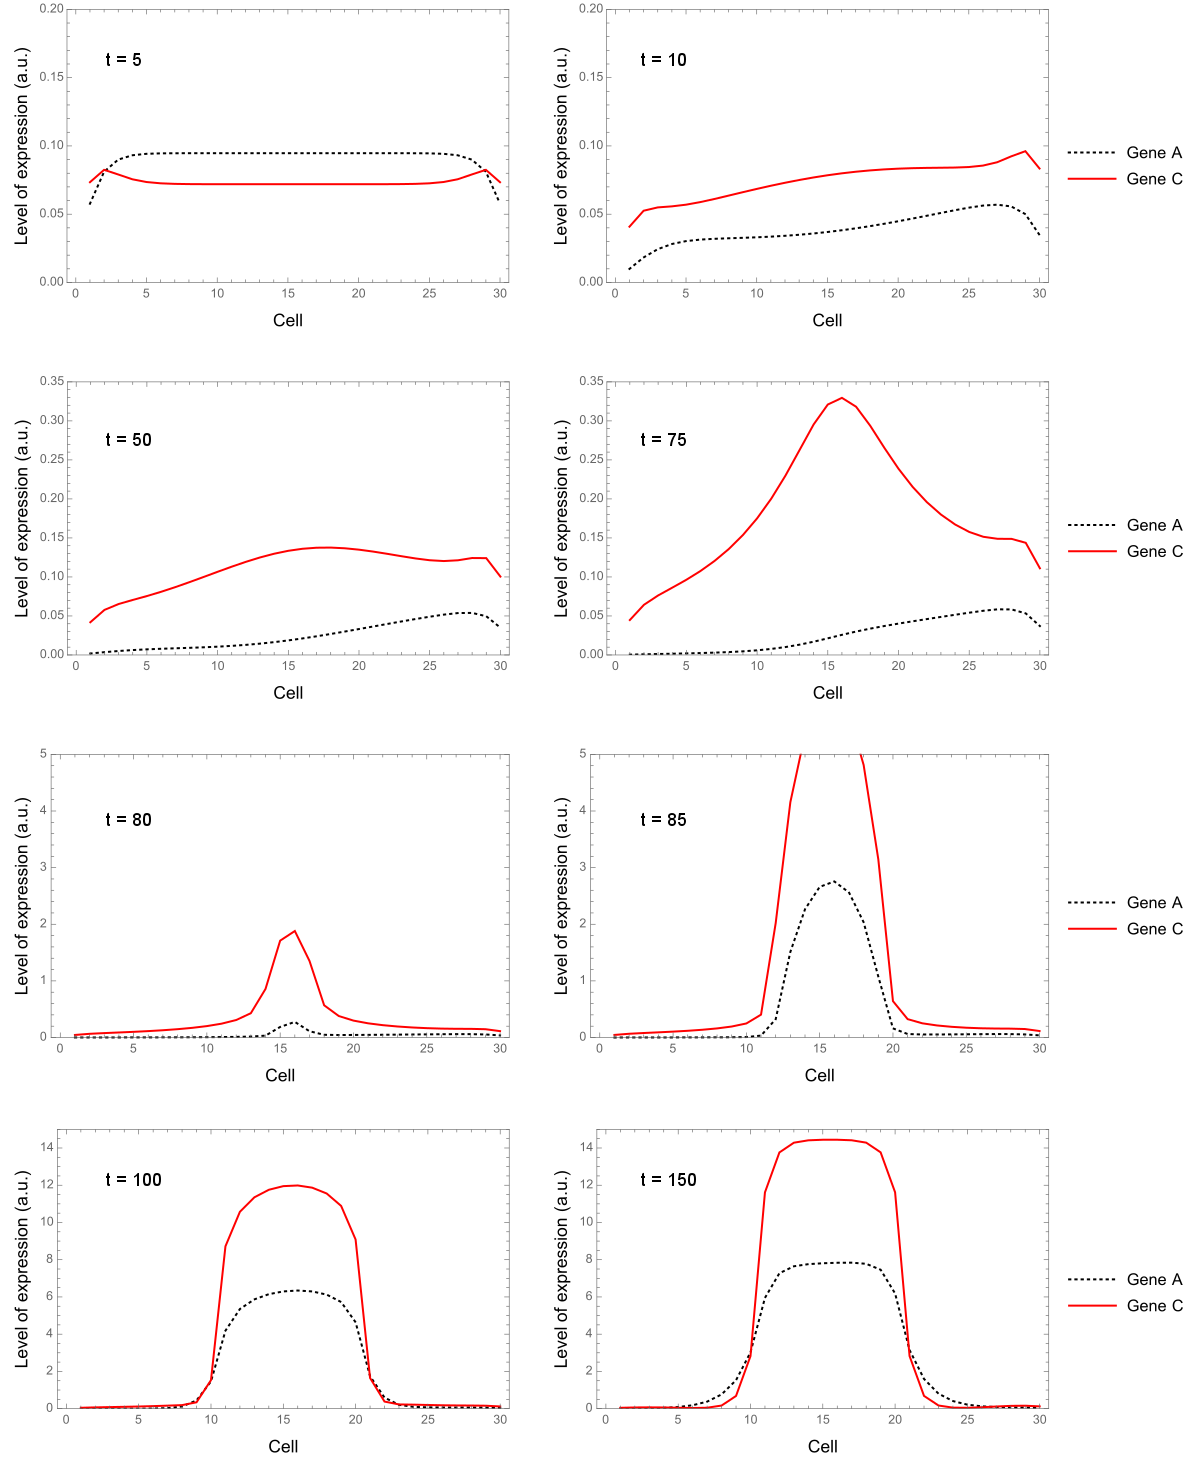
\includegraphics[width=\textwidth]{figures/results/topol-9-dynamics}
%  \caption{\bf Dynamics of expression in topology number 9.}
%  \label{fig:topol9-dyn}
% \end{figure}

In this way two bands of expression that depend on each other are formed. The
high level of gene C in the middle of the field counteract its inhibition by
gene A, while at the ends of the bands the inhibition of gene A on gene C
overcomes the self-activation of gene C, preventing the expression of the
latter to extend out of the middle of the field. In turn, the band of
expression of gene A can only exist in the middle of the field because its
expression depends on gene C.

This is a complex mechanism reminiscent of the Gierer-Meinhardt model, which
to the best of our knowledge is reported for the first time in the context of
multiple morphogen inputs, and could thus be of particular interest to for
synthetic biology implementations to assess the feasibility and robustness
conferred by this mechanism to GRNs.

\section*{Discussion}

In this work, we have conducted extensive computational explorations of small
GRNs with the capacity to generate a simple spatial pattern in a 1-D
morphogenetic field. Our findings shed new light on regulatory rules and
dynamical mechanisms that GRNs in nature could potentially implement to
achieve stereotyped spatio-temporal tasks.

Overall, based on our extensive search space exploration we identified
a great variety of pattern-forming GRN topologies  with distinctive and often
widely shared building blocks (network motifs), which are likely to confer
each topology the ability to achieve specific regulatory tasks in a semi-autonomous
manner. In particular, we uncovered a great variety of network
topologies that could produce a striped gene expression pattern, where 615 out of
714 were found to be multi-input topologies, which highlights the importance of
often disregarded pleiotropic signaling events as a potentially critical design
specification rule for successful synthetic biology implementations of GRNs
with various types of pattern-forming abilities. Most importantly, we found that
this ensemble of pattern-forming GRNs
tends to form a highly connected meta-graph, which highlights emergent
properties, such as robustness and evolvability, of complex biological
systems at a very high level~\cite{kitano2004}.\\

Robustness is a defining feature of any developmental patterning process.
Our results suggest that the underlying morphogen interpretation
mechanisms (GRNs) are highly accessible by exploring the
topology space constrained by selection for their final steady-state and
by their ability to buffer noise~\cite{lo_robust_2015, exelby_2021}.
In our study, the most abundant topologies were found forming highly
connected clusters in a so-called neutral network of genotypes,
implying that the corresponding GRN topologies would tend to be robust
to quantitative changes in the strength of regulatory interactions, diffusion, and
degradation parameters, as well as to qualitative changes in the topology
itself. In essence, such organization could be seen as an intrinsic evolutionary
property of GRNs that facilitates the coexistence of robustness and
evolvability~\cite{wagner_robustness_2008}. For instance, bridge topologies
in the neutral network connect distinct classes of pattern-forming
GRNs~(\nameref{S6_Fig}), suggesting that evolutionary transitions between
different GRNs (for example, between a Gierer-Meinhardt-like network to an
Incoherent Feed-Forward Loop) could be achieved with minimal fitness costs. This high-level
property of the neutral network of topologies could thus facilitate the fine-tuning
of the regulatory systems through genetic modifications to meet
specific functional requirements under selective pressures.

In contrast to this robustness to
qualitative and quantitative changes, we found that many GRNs were susceptible
to changes in morphogenetic field size. However, interestingly, GRNs with the same
topology behave in different ways for each field size~(\nameref{S3_Fig}C),
indicating that the specific values of network parameters are more important
than the network topology when it comes to producing the same pattern at
different scales.

Other studies have shown that Incoherent Feed-Forward Loops can form
spatial stripes of gene expression~\cite{ishihara_cross_2005}. In particular,
we found that the I3-FFL is one of the network motifs that appears more
frequently in these GRNs, which is in agreement with the study by Cotterell \&
Sharpe~\cite{Cotterell2010}, and has been found in transcriptional networks involved
in cell fate definition~\cite{Li2019}. Moreover, our results indicate that this
is a robust motif that can be useful for constructing synthetic gene
regulatory networks exposed to stochastic fluctuations in the
environment and mutations.

However, as our model was less stringent and allowed the morphogen input to
interact with any gene, we found a significantly larger number of pattern-forming
topologies, which can operate under disparate combinations of diffusion and degradation
parameters~(\nameref{S7_Fig}). For example, in a single input GRN model, the I4-FFL
has not been found capable of generating a striped gene expression
pattern~\cite{munteanu_2014}, whereas, in our experimental setup, 20.17\% of
the topologies were found  to implement such a regulatory motif~(\nameref{S1_Table}).

Although recent experimental evidence highlights the importance of the Incoherent
Feed-Forward Loop type 2 (I2-FFL) for generating a striped gene expression
pattern~\cite{Schaerli2014, Basu2005}, it is intriguing to find that such motif is
underrepresented in our study, with only 10.92\% of the topologies implementing
such regulatory mechanism. This might be due to the difficulty to find optimal
solutions when probing the design space of multi-input GRNs, which are likely to
contain multiple locally optimal solutions. In addition, it is important to mention
here that the application of a MCMC-like algorithm as a search space strategy for
such complex tasks cannot be expected to allow for extensive exploration of the
design space of GRNs nor for the accessibility of every single locally optimal
solution. However, it is also possible that the I2-FFL motif is not as robust as
other motifs and therefore be less represented.

We also found topologies with a similar topology to that of the “opposing
gradients” reported by Schaerli et al.~\cite{Schaerli2018,Schaerli2014}.
Although the “opposing gradients” mechanism requires the constitutive expression
of two of the genes in the GRN, and our model does not take constitutive
expression into account, we observed that the GRNs that implement the “opposing
gradients” mechanism also tend to implement auto-regulation interactions on
these two nodes, bypassing in this way the lack of constitutive
expression as found in previous studies~\cite{munteanu_2014}.

The correlation between the complexity index of a topology and its abundance
indicates that networks with simpler designs are more robust to changes in
interaction parameters and that more complex networks are less robust. For
example, topology number 420~(Fig~\ref{fig:2neut-net}), which
presents high complexity, was one of the
topologies with lower abundance and was disconnected from all other topologies
in the two-step neighbors in the neutral network.

Although GRNs that produce a band of gene expression with only two nodes have
been described (e.g., the I-zero motif~\cite{Schaerli2014}), this is to our
knowledge the first time that a novel GRN topology such as number
9~(Fig \ref{fig:topol9}) has been reported, which adds considerably to existing
knowledge on the genotype-phenotype mapping problems studied in the
context of developmental pattern formation. It would be interesting to assess
experimentally the ability of this particular topology to generate striped gene
expression patterns, as well as to assess its robustness in the face of mutational
changes and noisy morphogen input profiles.

Overall, we believe our work provides a set of enticing hypotheses on GRN designs,
represented as a large catalog of distinct GRN topologies that could provide
valuable information as starting points for future computational and theoretical
analysis of the genotype-phenotype map, as well as for experimental validation and
future discovery of potentially interesting GRN designs.

%\section*{Conclusion}

\section*{Supporting information}

% Include only the SI item label in the paragraph heading. Use the \nameref{label} command to cite SI items in the text.

\paragraph*{S1 Fig.}
\label{S1_Fig}
{\bf Most GRNs reach the steady state before 250 time steps.}
(A) Gene regulatory network displaying the topology number 33. (B) Spatiotemporal
expression profile of the gene regulatory network shown in (A).

\paragraph*{S2 Fig.}
\label{S2_Fig}
{\bf Relevant subgraphs present in the set of GRNs.}
These are subgraphs that have been reported in previous studies as networks
involved in morphogenesis and development~\cite{Cotterell2010, Schaerli2014,
Schaerli2018}. These were used to calculate the subgraph profile and the results
reported in \nameref{S1_Table}.

\paragraph*{S3 Fig.}
\label{S3_Fig}
{\bf Response of GRNs to changes in morphogenetic field size.}
(A) Morphogen gradients of fields with 10, 20, 40 and 50 cells. (B) Fitness of the
GRNs by topology in each one of the morphogenetic fields. (C) Principal Component
Analysis of fitness by morphogenetic field size. Although principal components
separate GRNs in clusters, not all the GRNs with the same topology are located in the
same group. (D) Average fitness of GRNs evolved in different morphogenetic
field sizes.

\paragraph*{S4 Fig.}
\label{S4_Fig}
{\bf Expression dynamics of main networks.}
The dynamics of expression is shown from $t = 1$ to $t = 30$ for the eight most
abundant topologies. The red line
represents the expression level of the gene C along the morphogenetic field,
the blue line represents the expression level of gene B and
the dotted line represents the expression level of gene A.

\paragraph*{S5 Fig.}
\label{S5_Fig}
{\bf Dynamics of expression of topology number 9.}
The dynamics of expression is shown from $t = 5$ to $t = 150$. The red line
represents the expression level of the gene C along the morphogenetic field,
whereas the dotted line represents the expression level of gene A. The
striped pattern of gene expression can be seen for both genes since $t = 80$.

\paragraph*{S6 Fig.}
\label{S6_Fig}
{\bf Bridge topologies in the neutral network.}
``Bridge topologies'' are those topologies that connect two clusters in the neutral
network (Fig~\ref{fig:neutral-network}), and as such can be interpreted as
intermediary steps in the evolution from a cluster of related topologies into
another cluster. For example the topology 441 could be an initial step to reach the
topology 9, as in this topology nodes B and C are not connected.

\paragraph*{S7 Fig.}
\label{S7_Fig}
{\bf Diffusion and degradation parameters.}
(A) Ternary plot showing the combination of diffusion parameters for genes A,
B and C. (B) Ternary plot showing the combination of degradation parameters
for genes A, B and C. The color gradient that goes from topology 1 in white to
topology 714 in black shows no distinguishable pattern.

\paragraph*{S1 Appendix.}
\label{S1_Appendix}
{\bf Diffusion independent networks and robustness to changes in the signal input.}

\paragraph*{S1 Table.}
\label{S1_Table}
{\bf Proportion of relevant subgraphs in the set of GRNs.}
The 19 subgraphs presented in this table are those presented in \nameref{S2_Fig}.
Most of the topologies presented at least one negative feedback loop (70.73\%),
and 62.46\% of them presented the I3-FFL network motif. The robustness of each
subgraph was calculated as the mean robustness of the topologies presenting that
subgraph.

\paragraph*{S2 Table.}
\label{S2_Table}
{\bf Average fitness of each topology in different morphogenetic fields.}
The average fitness by topology is reported for morphogenetic fields with 10, 20,
40 and 50 cells. Data from this table are shown in \nameref{S3_Fig}B.

\section*{Acknowledgements}
The computational resources (Stevin Supercomputer Infrastructure) and
services used in this work were provided by the VSC (Flemish Supercomputer
Center), funded by Ghent University, FWO and the Flemish Government–department EWI.
All authors acknowledge partial support from CoDI-Universidad de Antioquia under
project ``Estudio de la Evolución de Circuitos de Regulación del Desarollo Embrionario a través de
la Biología Evolutiva de Sistemas'' code 2017-14367. All authors acknowledge the Colombian
youth for their defense of a better country.

\nolinenumbers

% Either type in your references using
% \begin{thebibliography}{}
% \bibitem{}
% Text
% \end{thebibliography}
%
% or
%
% Compile your BiBTeX database using our plos2015.bst
% style file and paste the contents of your .bbl file
% here. See http://journals.plos.org/plosone/s/latex for
% step-by-step instructions.
%
% \begin{thebibliography}{10}
%
% \bibitem{bib1}
% Conant GC, Wolfe KH.
% \newblock {{T}urning a hobby into a job: how duplicated genes find new
%   functions}.
% \newblock Nat Rev Genet. 2008 Dec;9(12):938--950.
%
% \bibitem{bib2}
% Ohno S.
% \newblock Evolution by gene duplication.
% \newblock London: George Alien \& Unwin Ltd. Berlin, Heidelberg and New York:
%   Springer-Verlag.; 1970.
%
% \bibitem{bib3}
% Magwire MM, Bayer F, Webster CL, Cao C, Jiggins FM.
% \newblock {{S}uccessive increases in the resistance of {D}rosophila to viral
%   infection through a transposon insertion followed by a {D}uplication}.
% \newblock PLoS Genet. 2011 Oct;7(10):e1002337.
%
% \end{thebibliography}

\bibliography{referencias-tesis}{}

\end{document}
